\begin{figure}[ht]
	\centering
	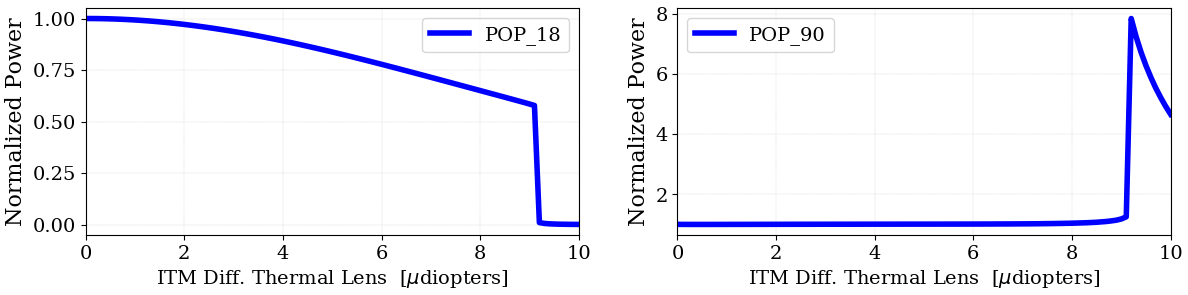
\includegraphics[width=1.0 \textwidth]{../Figures/POP18_POP90_DiffLens.png}
	\caption[Model of POP-18 as a function of differential thermal lensing.]  
	{\textbf{Model of POP-18 as a function of differential thermal lensing.}
		The horizontal axis is differential lensing between the ITMX/ITMY substrates and the vertical axis represents the normalized power when locked with nominal mode matching.  POP-18 is the signal at the power recycling pick-off port demodulated at 18 MHz which shows the sideband power buildup in the power recycling cavity.  Even with modest differential lensing (9 microdiopters), the buildup drops by 40 percent and eventually the simulation has trouble maintaining resonance, not too dissimilarly from the actual interferometer. 
	}
	\label{fig:POP18_POP90}
\end{figure}

\begin{figure}[ht]
	\centering
	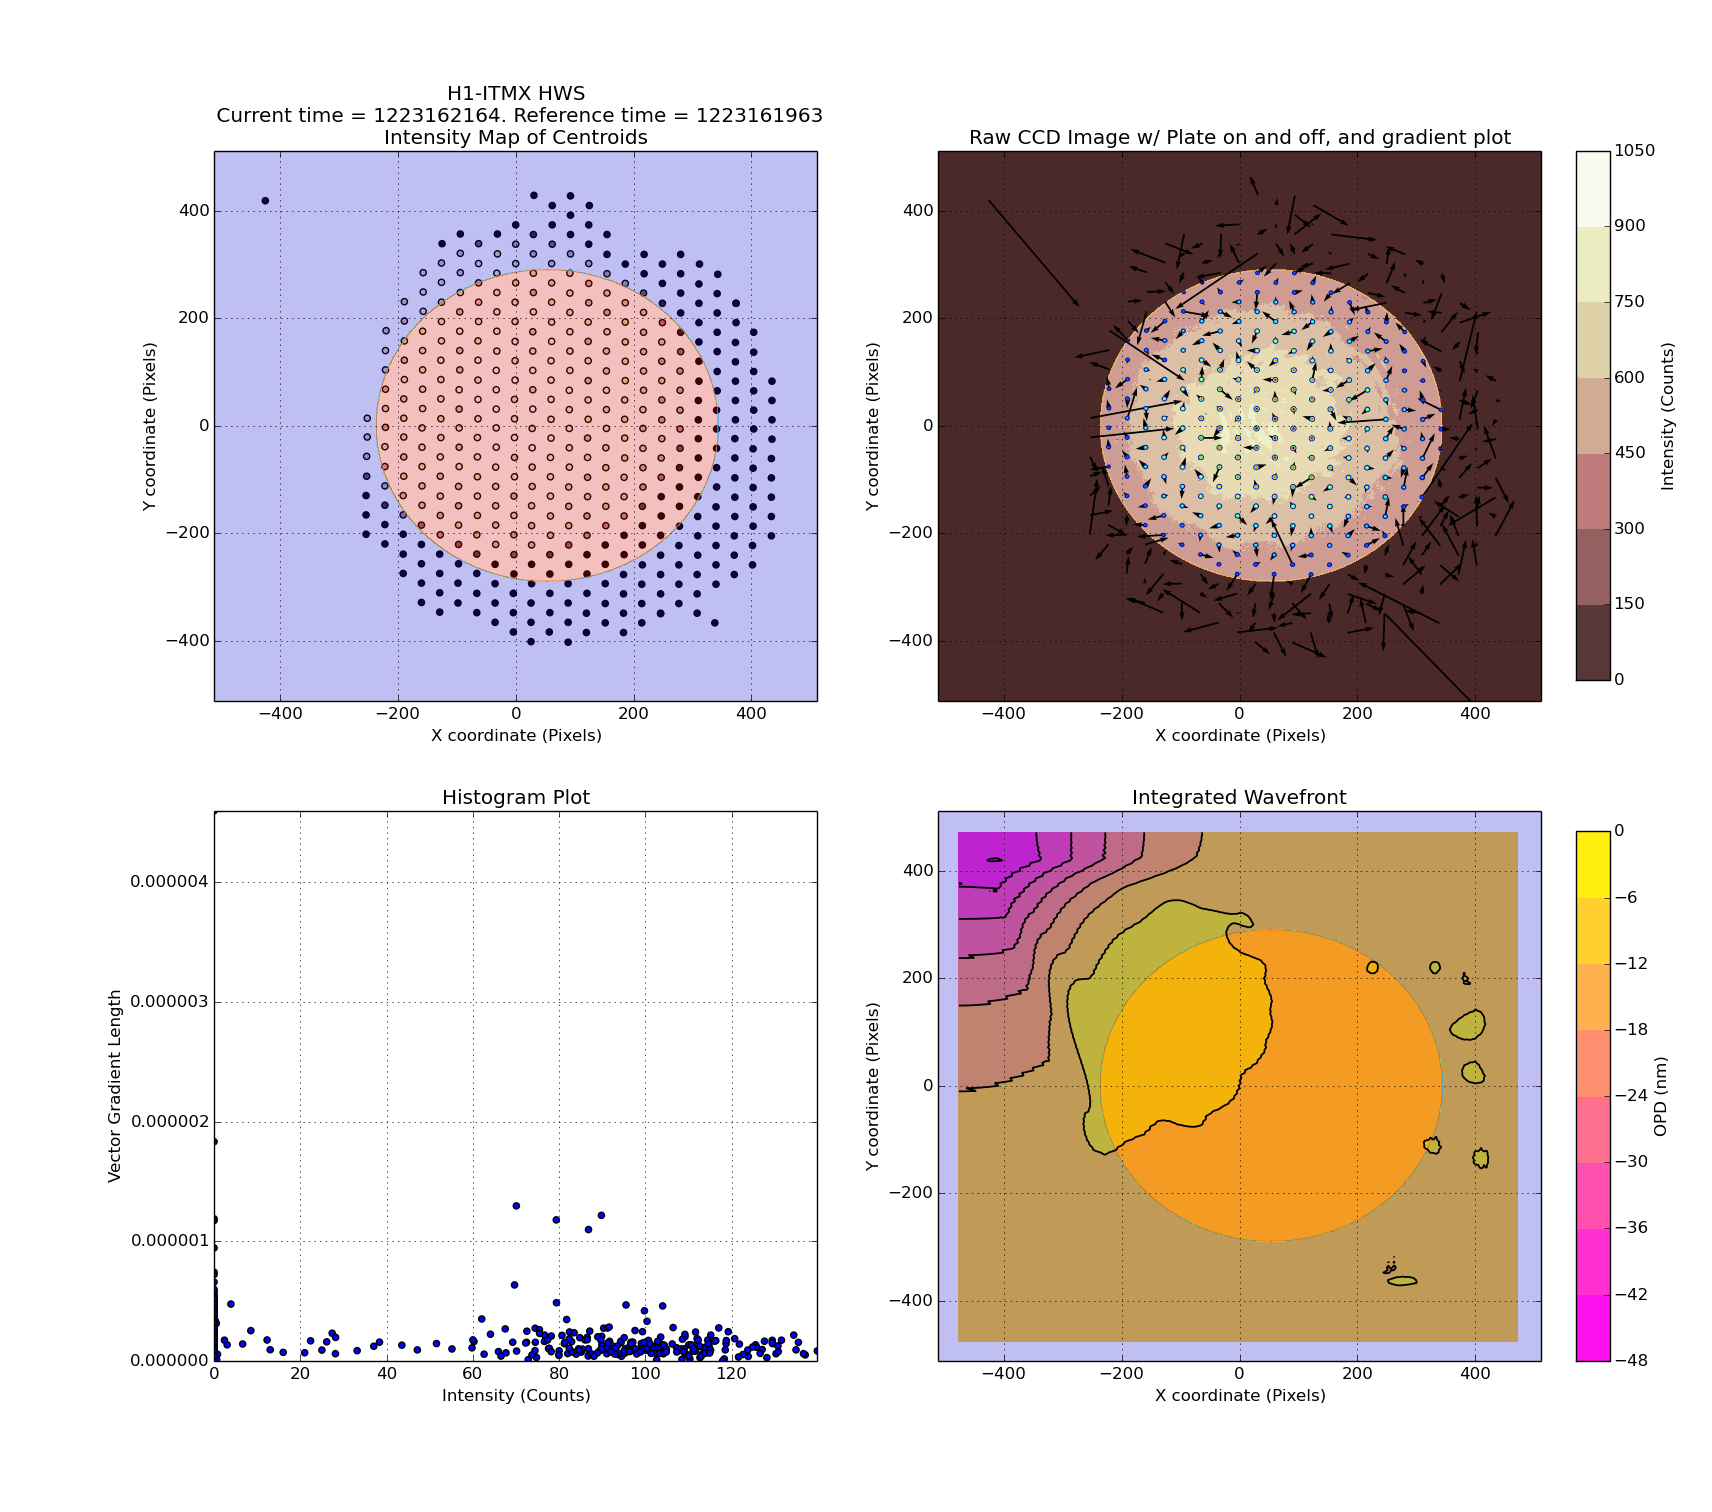
\includegraphics[width=0.7\textheight]{../Figures/20181011_ITMX_HWS_histogram_Masked.png}
	\caption[ITMX Hartmann Sensor output.] 
	{\textbf{ITMX Hartmann Sensor output.} Between the reference and current times for this measurement, no heating was applied to the test masses so the expectation is a relatively flat and smooth wavefront. This is mostly true except for a large, anomalous arrow at pixel coordinate [X,Y] = [-410, 405] of the gradient plots (upper right) which leads to a false wavefront distortion in the same area for the contour plot (lower right).  The sharp iris in the middle represents a digital mask that is can be turned on to reduce the effects of fringing.  A histogram in the bottom left plot shows the intensity distribution for each of the gradients; if the HWS beams are co-aligned well with the interferometer beam, then most of the information about thermal lensing occurs near the center of the intensity distribution.}
	\label{fig:HWS_Histogram}
\end{figure}

\begin{figure}[ht]
	\centering
	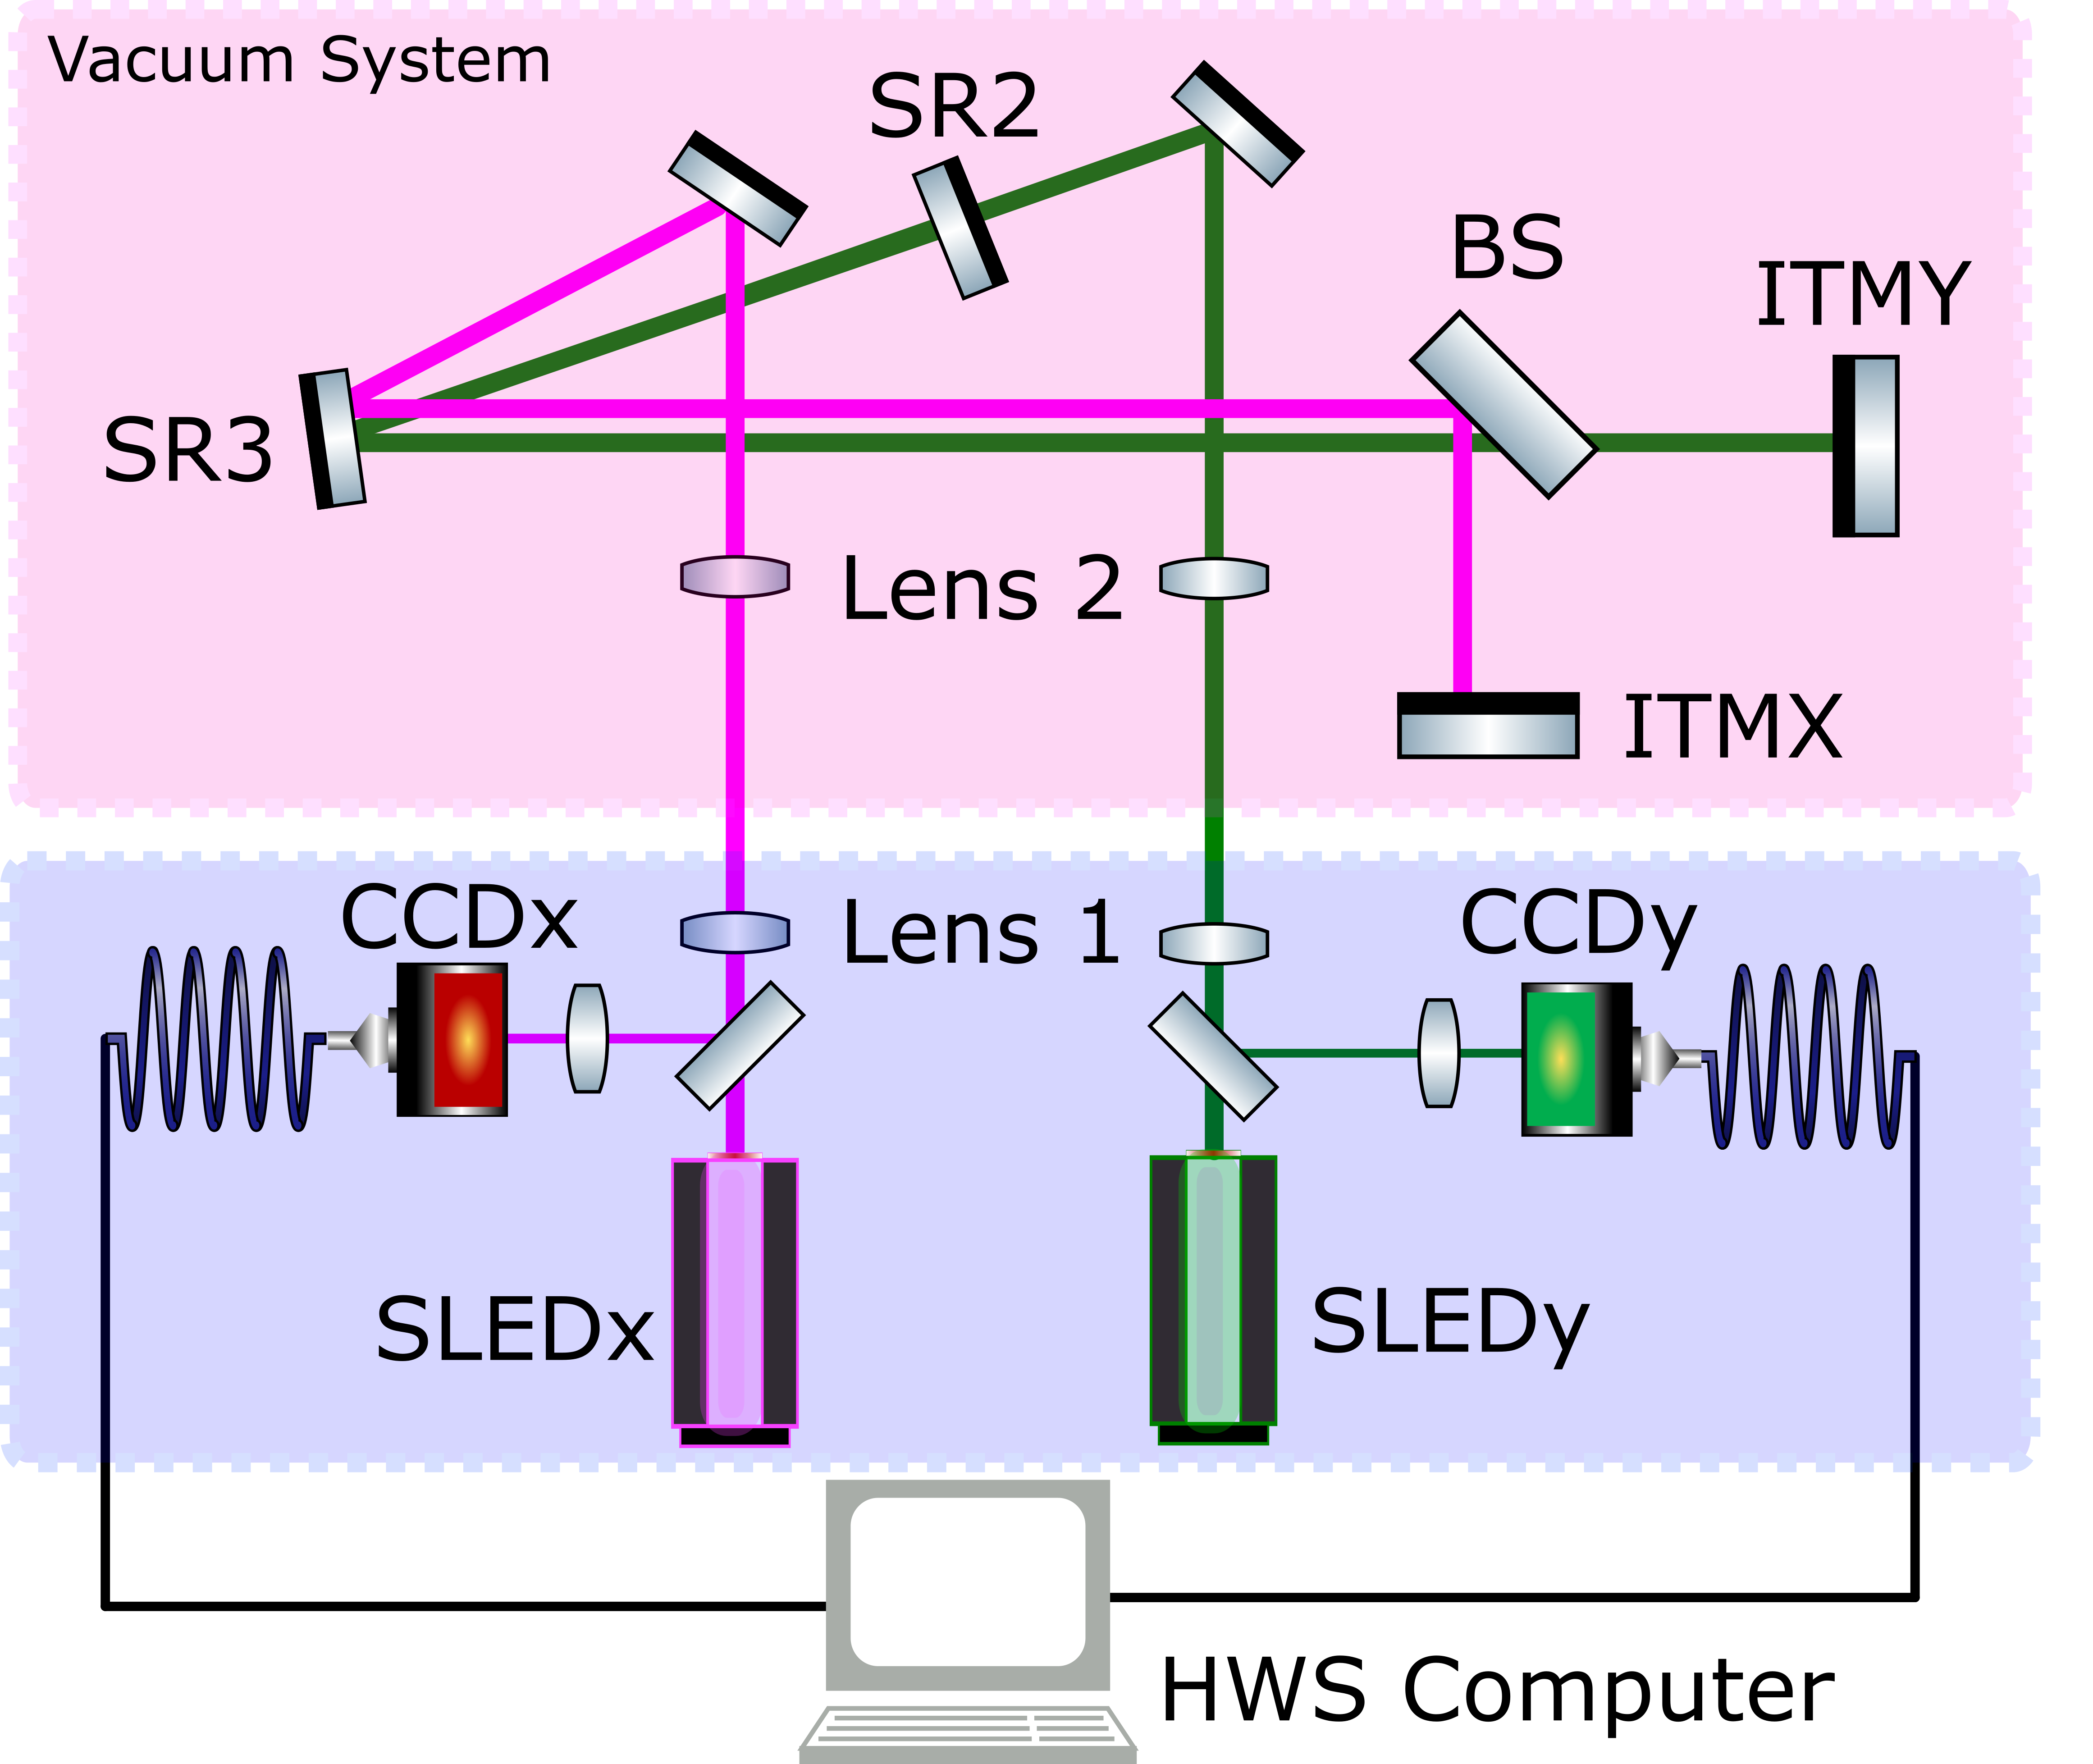
\includegraphics[width=0.6\textheight]{../Figures/HWS_OpticalLayout.png}
	\caption[ITM Hartmann sensors optical layout.] 
	{\textbf{ITM Hartmann sensors optical layout.} The path for injection is different for the two Hartmann sensors which use separate wavelengths to take advantage of the main beamsplitter AR/HR surface reflectivity. The ITMX (magenta) and ITMY (green) probe beam wavelengths are 800 nm and 833 nm, respectively, and have a 40 nm linewidth \cite{AWC_current}. The beams are sent into the vacuum system and retro-reflected off their respective optics back towards the pick-off mirrors before going into the CCDs with a Hartmann plate attached.  The cameras are then sent via fiber to a computer that runs the analysis pipeline on the images and exports the data to EPICS so the users can interface with the real time digital system in the control rooms.}
	\label{fig:HWS_optical}
\end{figure}

\begin{figure}[ht]
	\centering
	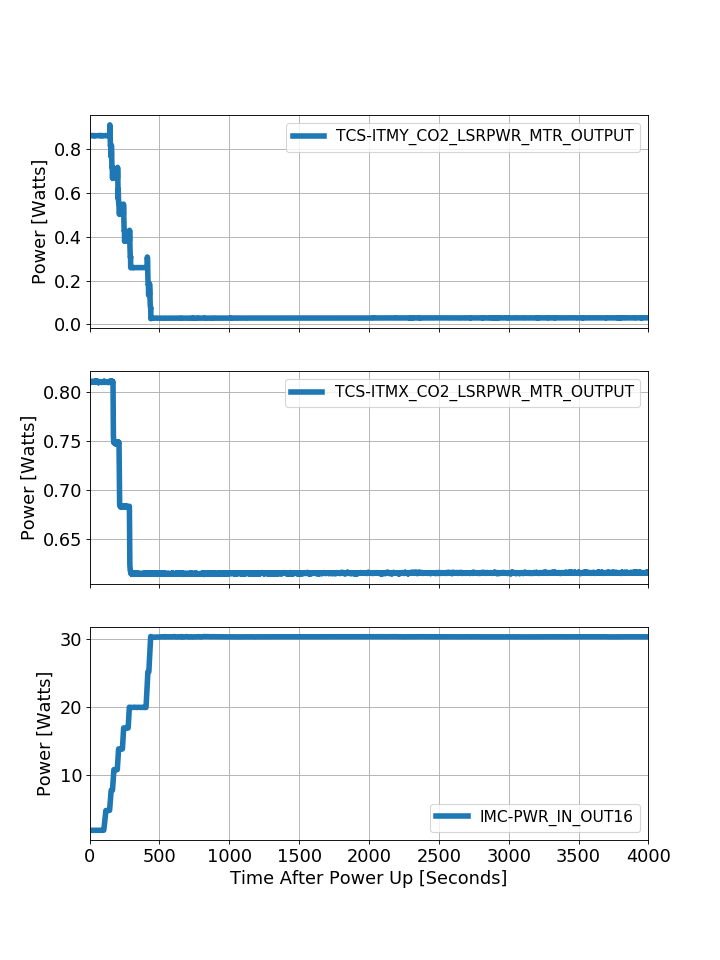
\includegraphics[width=0.35\textheight]{../Figures/1231726400TCS_and_PSL_powerup.png}
	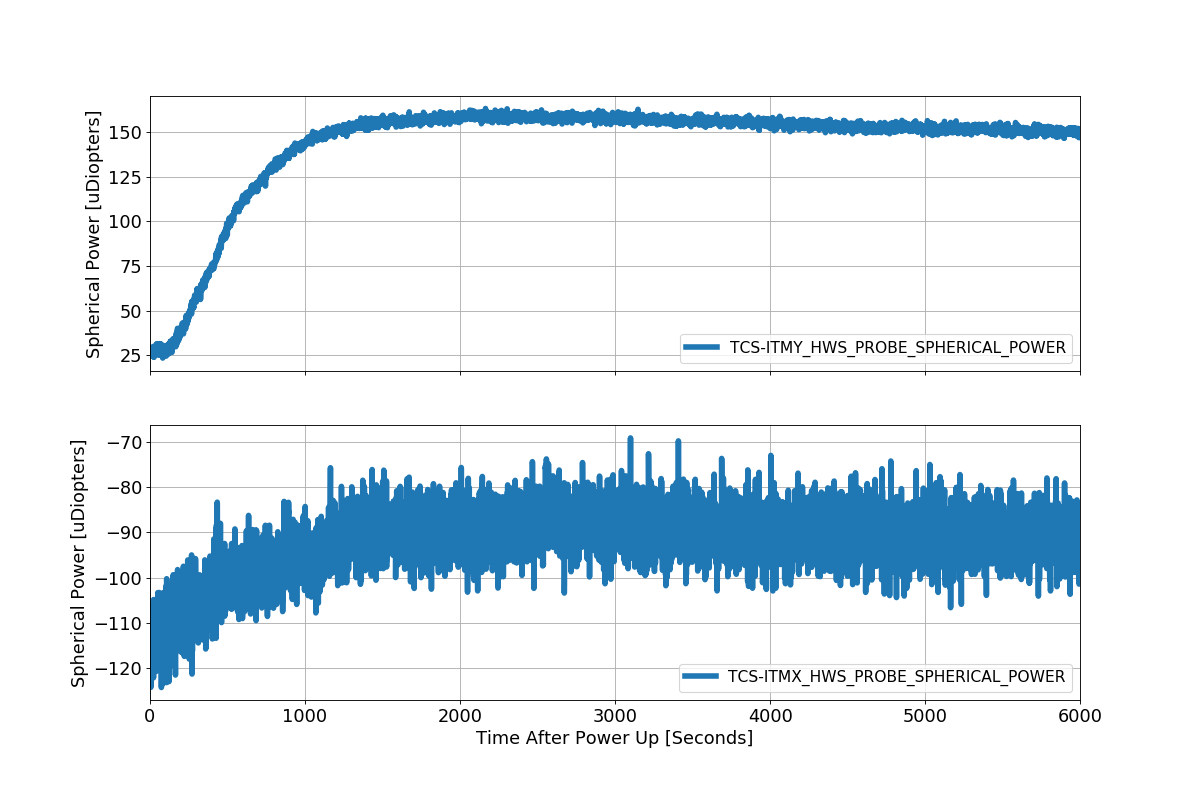
\includegraphics[width=0.35\textheight]{../Figures/1231726400HWS_powerup.png}
	\caption[A time series of the interferometer power increase sequence.] 
	{\textbf{A time series of the interferometer power increase sequence.} During this time, the interferometer is using DC-readout and locked at 2 watts of PSL input power with all of the angular control loops closed with high-bandwidth, in this configuration, the power recycling gain is approximately 45.  The left figure shows the increase of PSL input power and the CO2 lasers stepping down in power where levels of compensation were experimentally such that the angular control loops remain stable.  The right plot shows the Hartmann sensor spherical power as a function of time with the starting point scaled to zero micro-diopters.  Although the point absorbers do not exhibit the same spatial structure as uniform heating so it is difficult to derive absolute absorption for ITMY, the spherical fitting gives some information about the relative scale of heating absorption between the two optics.}
	\label{fig:pwr_up_time}
\end{figure}


\begin{figure}[ht]
	\centering
	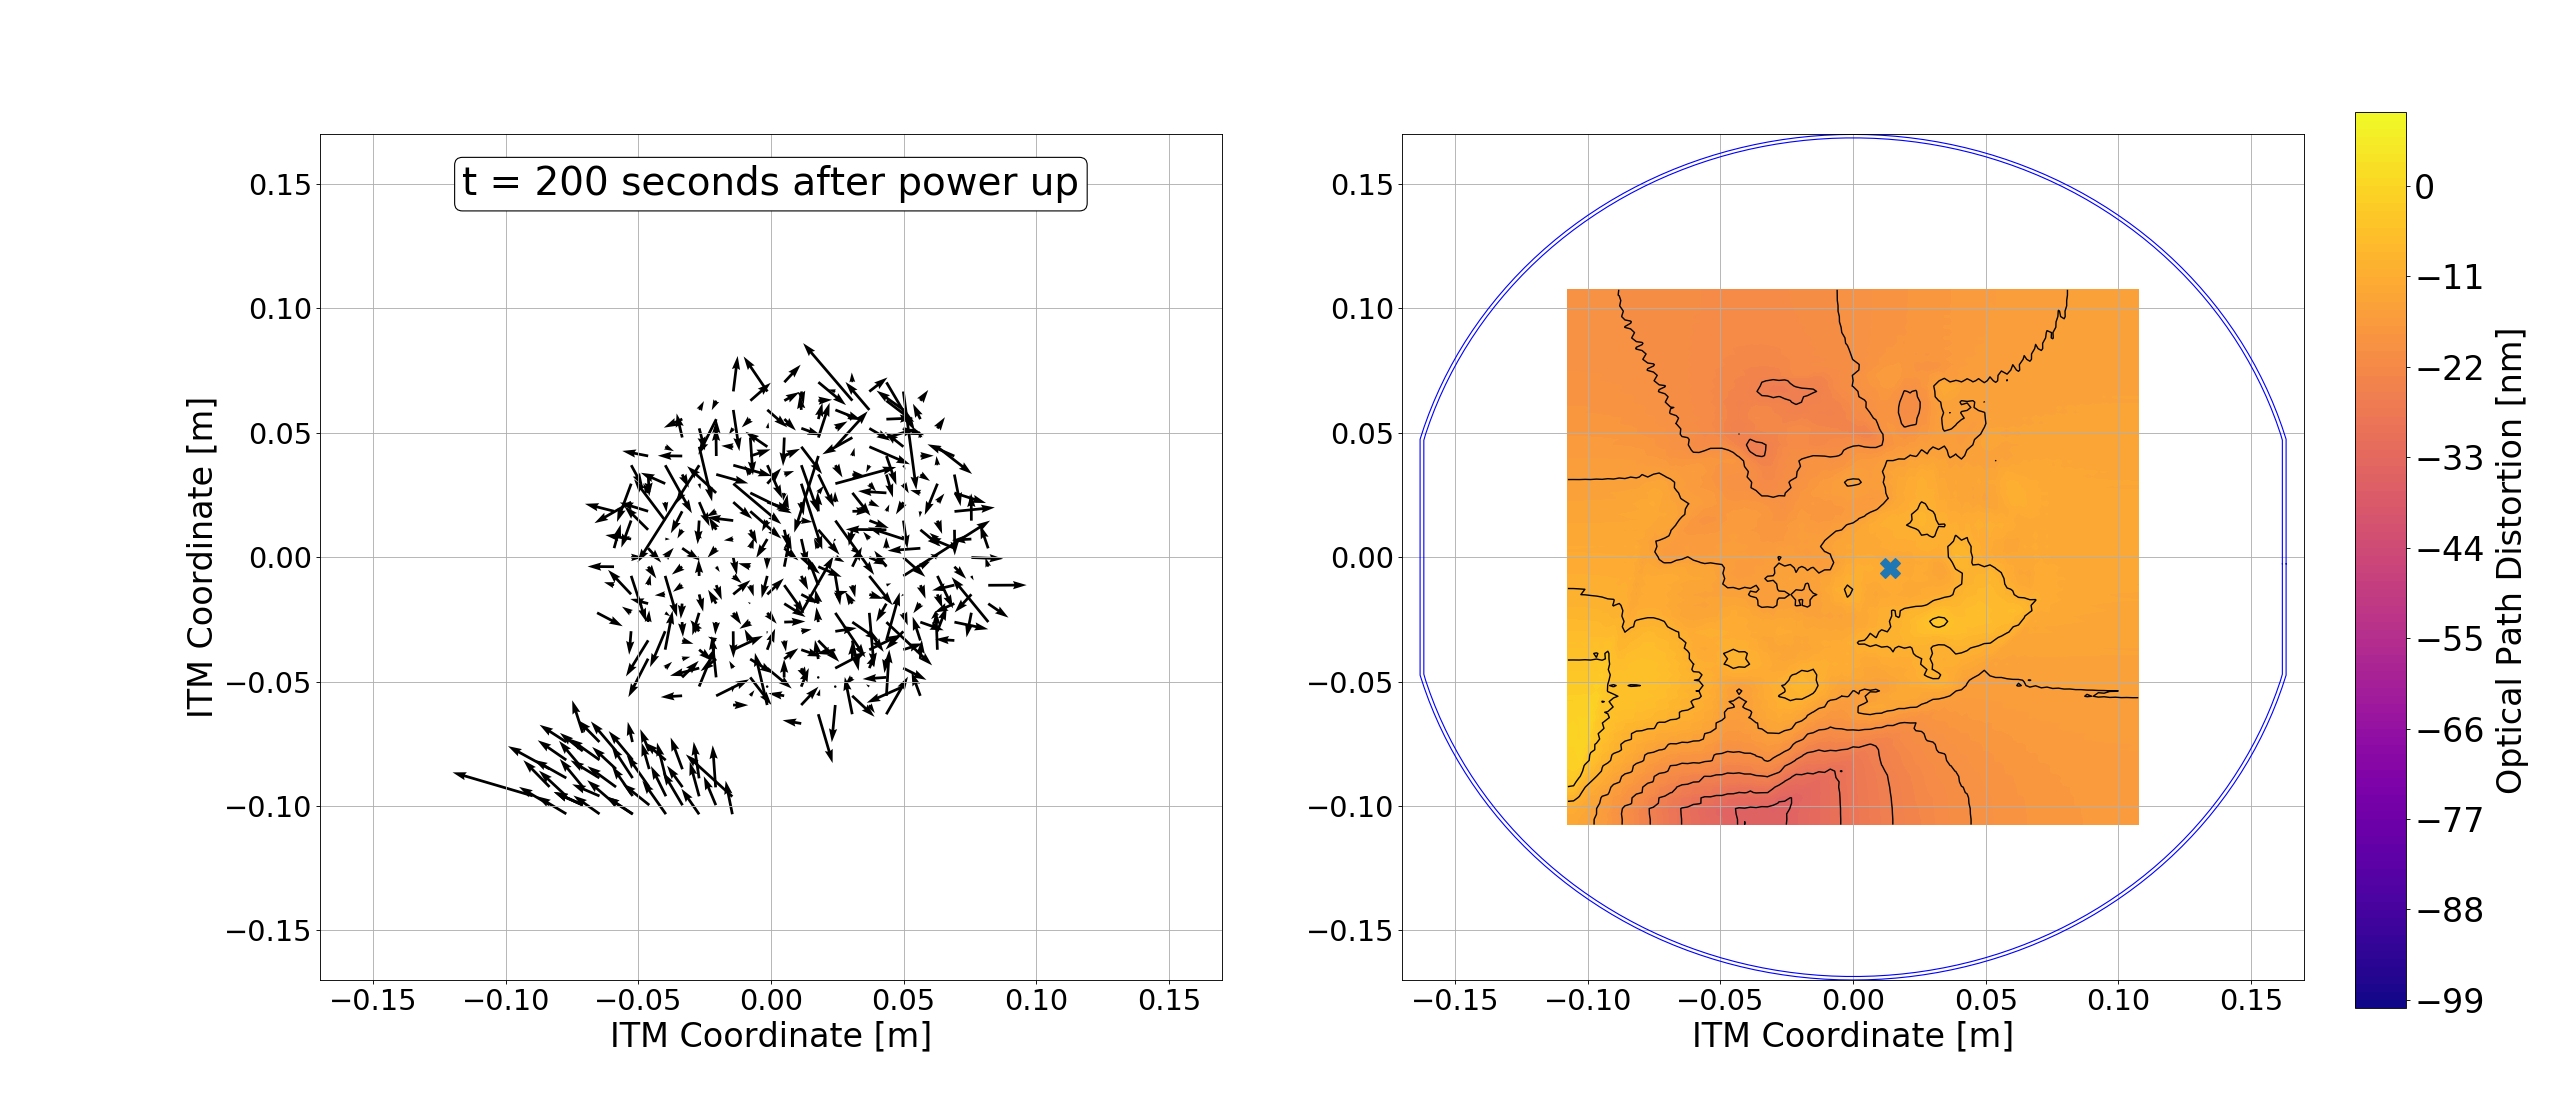
\includegraphics[width=0.5\textheight]{../Figures/1231726400_200dur_30W_ITMx.png}\quad
	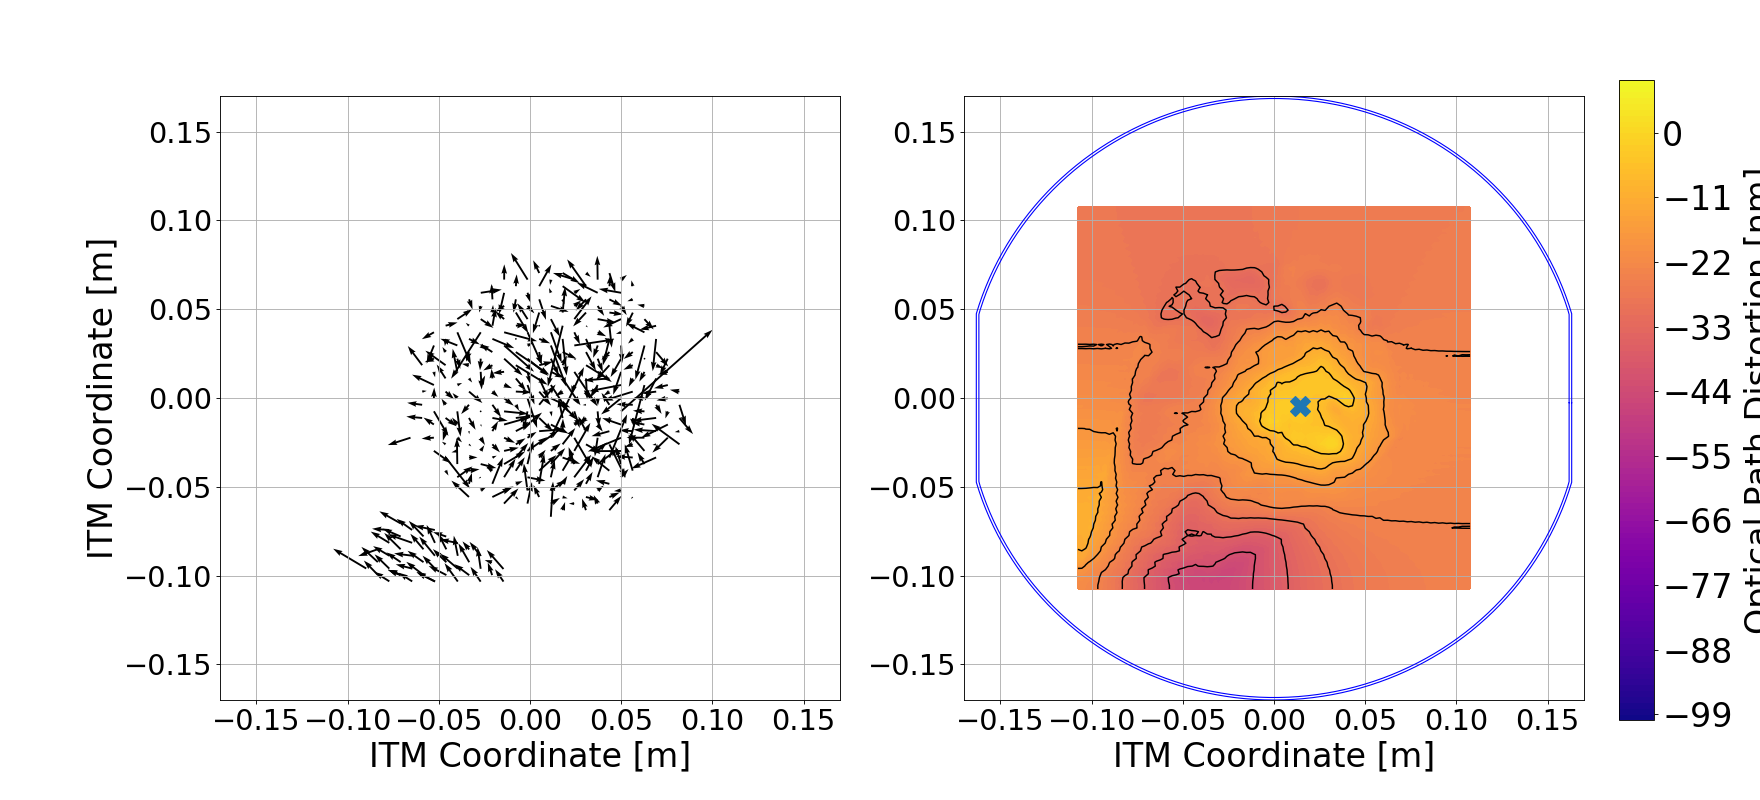
\includegraphics[width=0.5\textheight]{../Figures/1231726400_500dur_30W_ITMx.png}\quad
	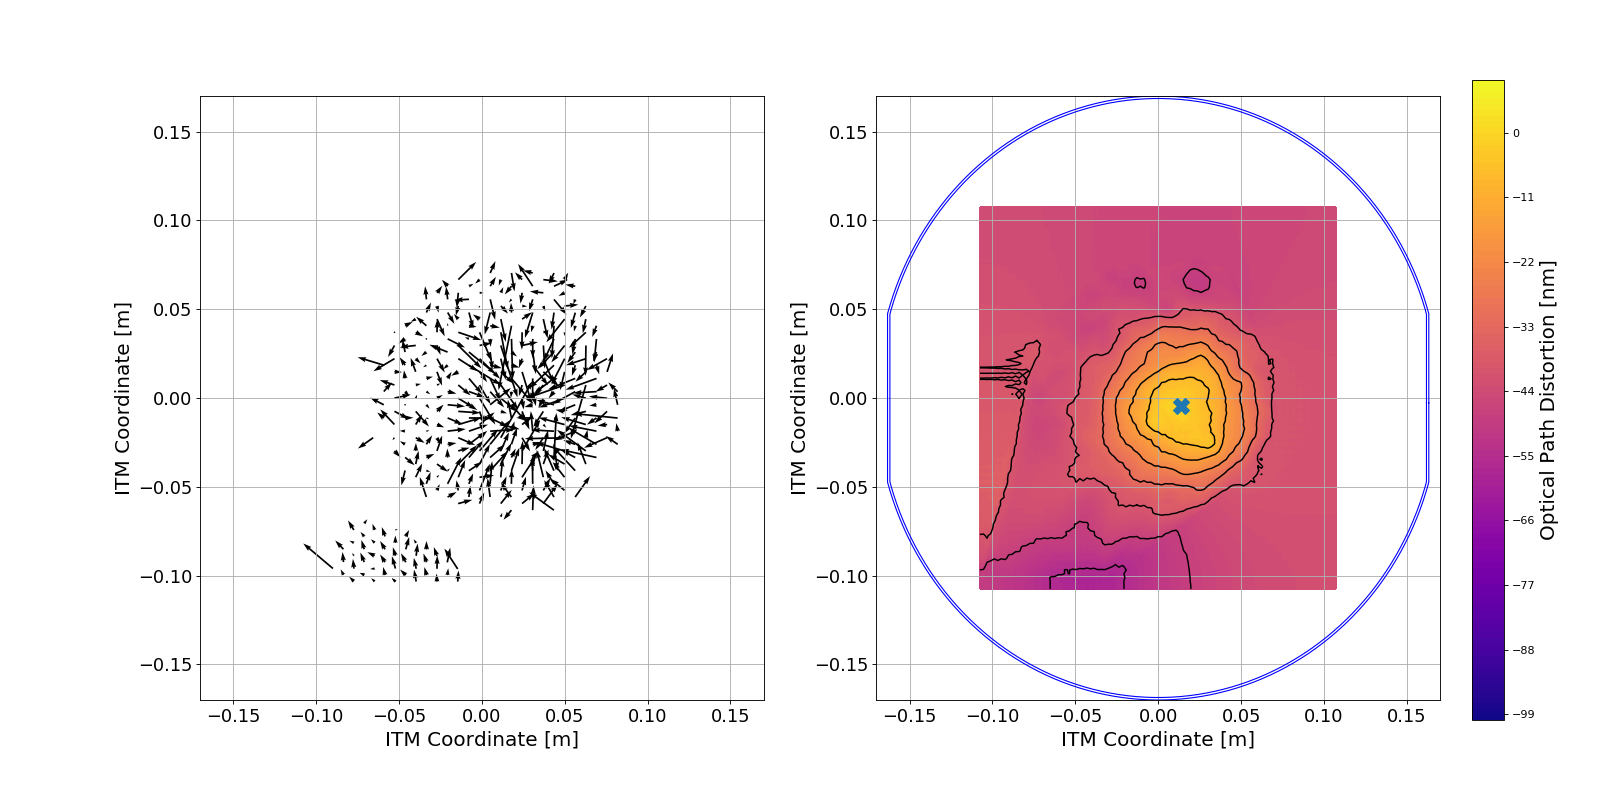
\includegraphics[width=0.5\textheight]{../Figures/1231726400_1000dur_30W_ITMx.png}\quad
	\caption[ITMX gradient plots (left) and wavefront maps (right) during a power up to 30 Watts of input power.]  
	{\textbf{ITMX gradient plots (left) and wavefront maps (right) during a power up to 30 Watts of input power.}
	It is important to note that there is a back-reflected stray beam from the super-luminous LED that is incident in the bottom left portion of the camera which is digitally cropped out during the real-time analysis. As previously noted, this particular Hartmann sensors suffers from beam clipping on the right side of the image which adds to the systematic noise.  A blue cross denotes the origin which is fitted with the Zernike polynomials to derive a spherical power.  The arrow lengths in the gradient plots are normalized to each individual plot and are meant to guide the eye in discerning the directionality and pattern of lensing.}
	\label{fig:ITMX_HWS_plot}
\end{figure}

\begin{figure}[ht]
	\centering
	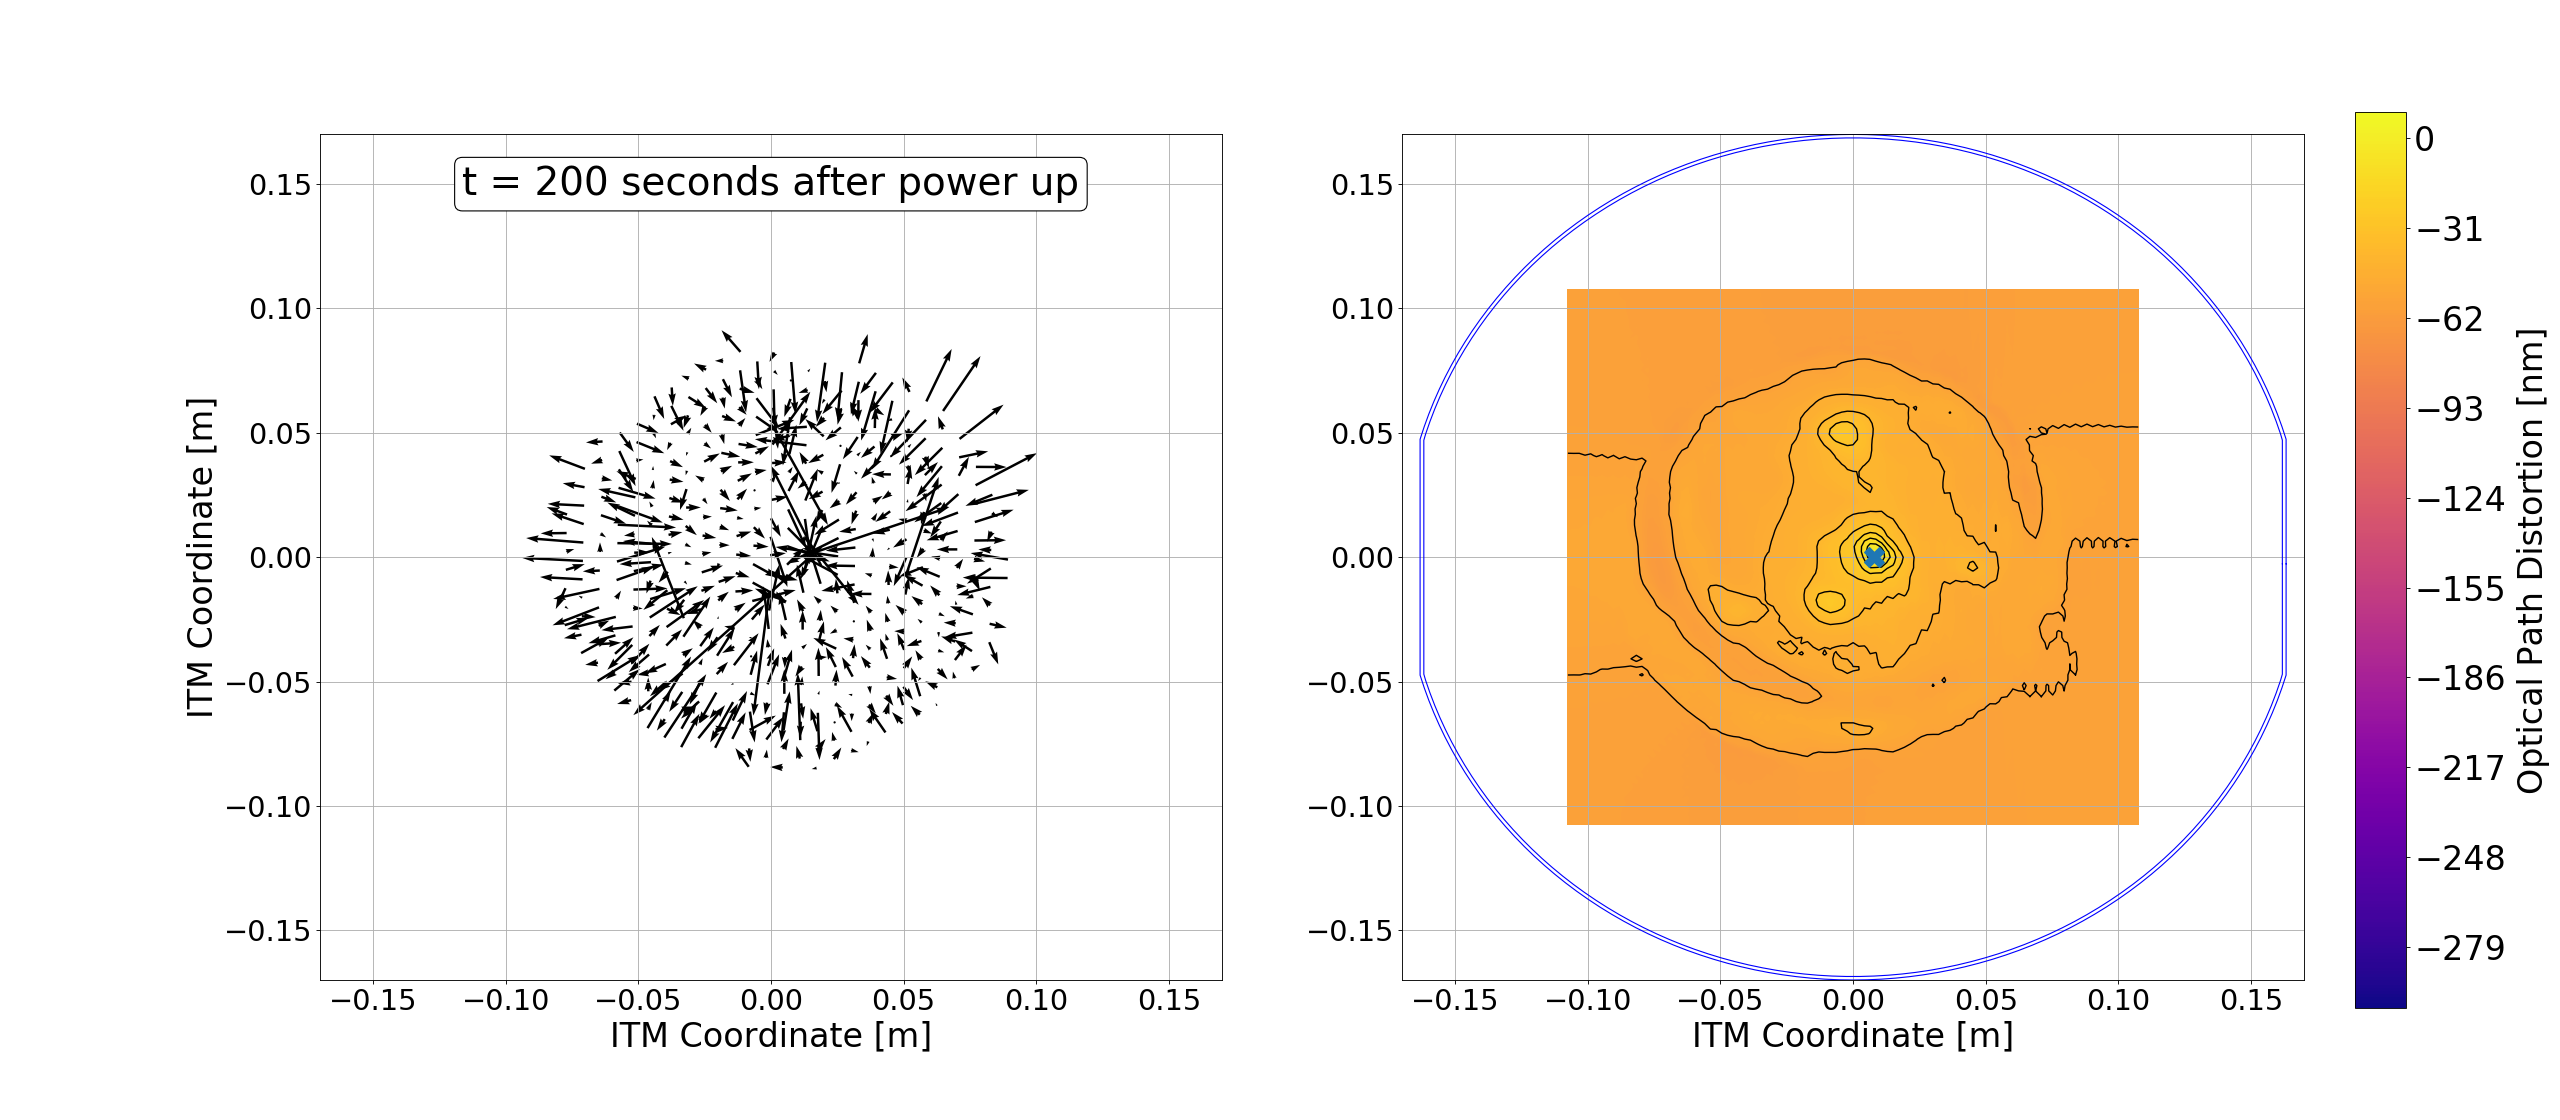
\includegraphics[width=0.5\textheight]{../Figures/1231726400_200dur_30W_ITMy.png}\quad
	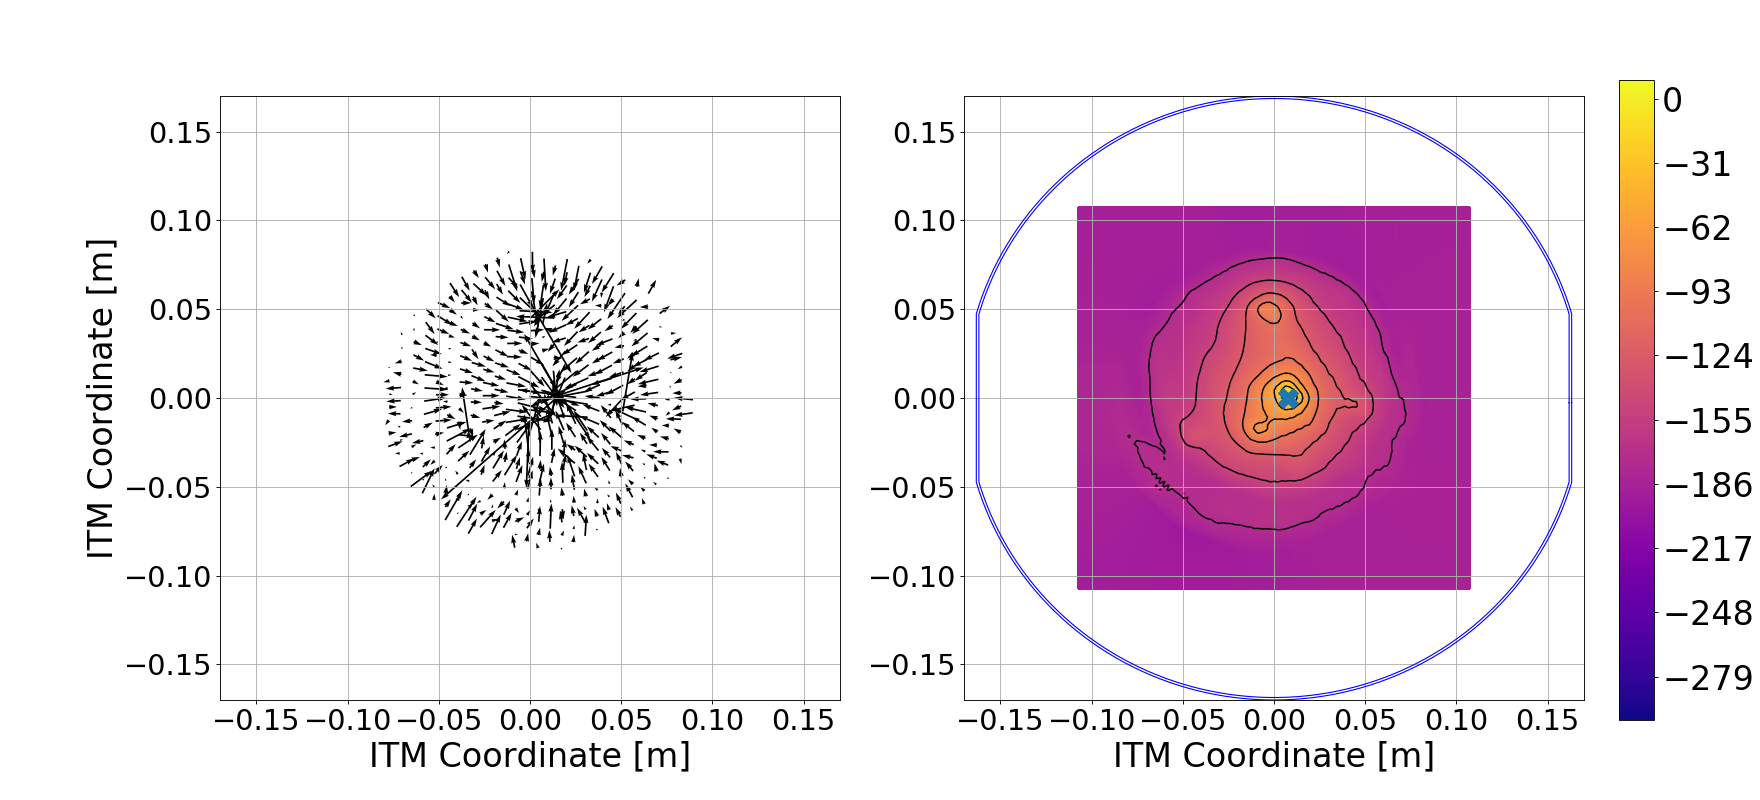
\includegraphics[width=0.5\textheight]{../Figures/1231726400_500dur_30W_ITMy.png}\quad
	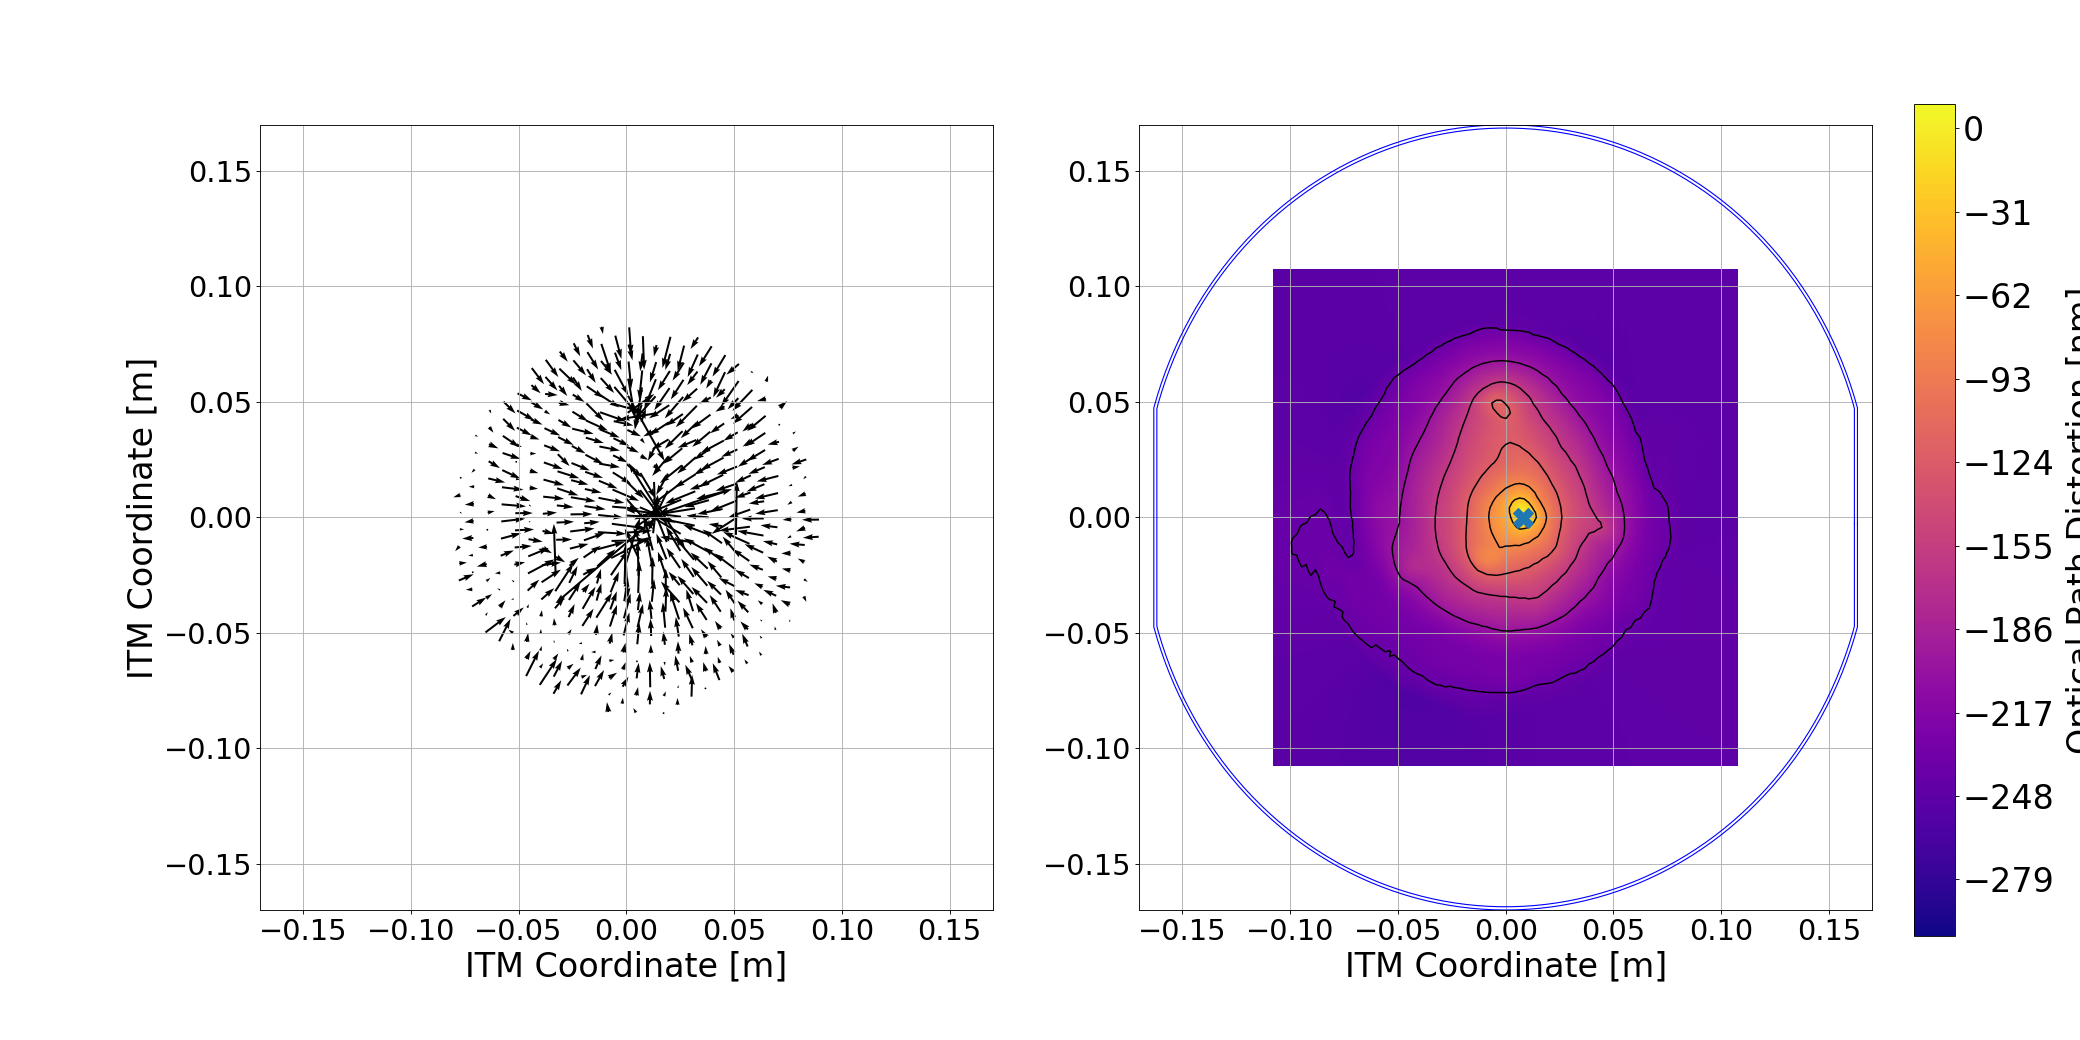
\includegraphics[width=0.5\textheight]{../Figures/1231726400_1000dur_30W_ITMy.png}\quad
	\caption[ITMY gradient plots (left) and wavefront maps (right) during a power up to 30 Watts of input power.]  
	{\textbf{ITMY gradient plots (left) and wavefront maps (right) during a power up to 30 Watts of input power.}
	Compared to the ITMX phase map in Figure \ref{fig:ITMX_HWS_plot}, ITMY has a much larger overall heating pattern and higher spatial frequencies in the contours which was the first clue that revealed multiple (possibly 4) point absorber on the test mass.  There is also a halo of gradients on the outer rim of the plots which is most prominent on the lower left corner.  This is due reducing the CO2 laser power in an attempt to compensate the lensing effects as the interferometer beam heats up the test mass.  The overall scale of self-heating with the higher spatial frequencies of the point absorbers makes it incredibly difficult to compensate with using the CO2 lasers as designed by Advanced LIGO. }
	\label{fig:ITMY_HWS_plot}
\end{figure}


\begin{figure}[ht]
	\centering
	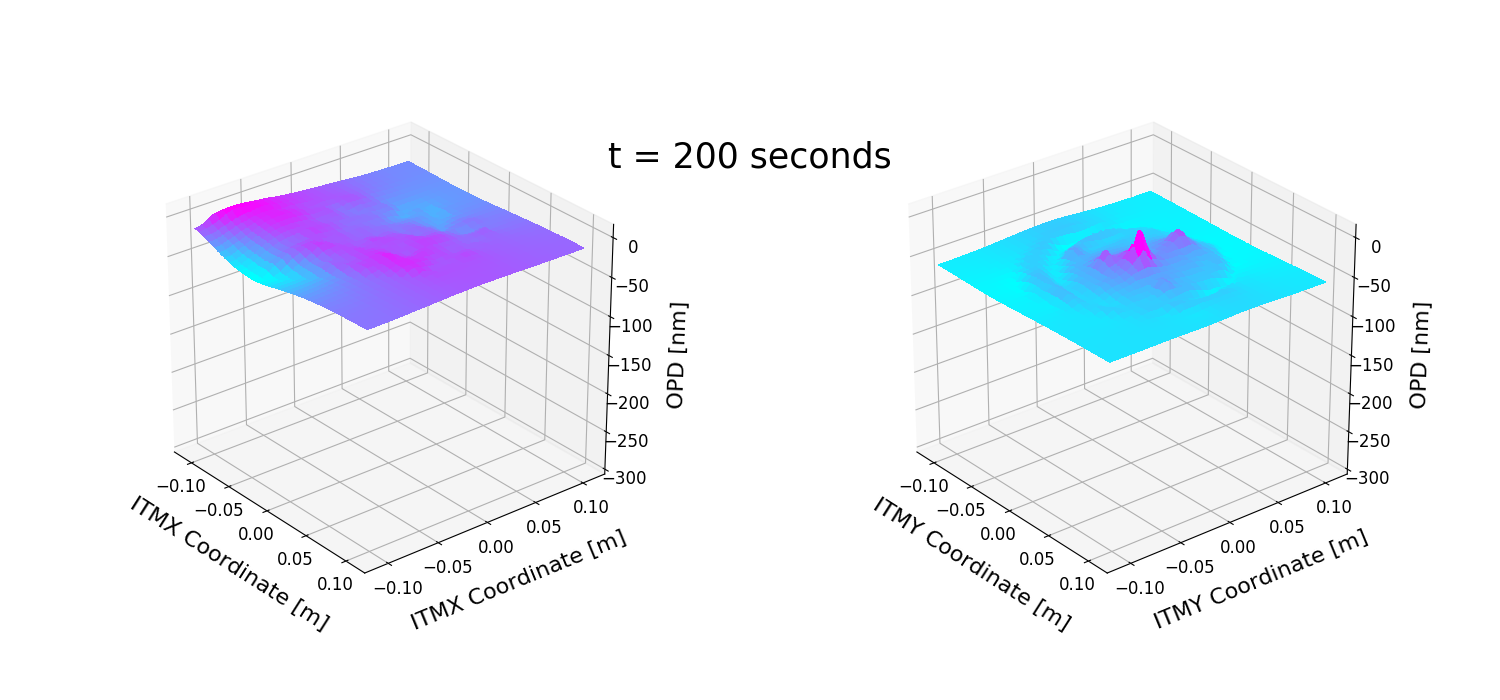
\includegraphics[width=0.4\textheight]{../Figures/1231726400_3d_200dur_30W_ITM.png}\quad
	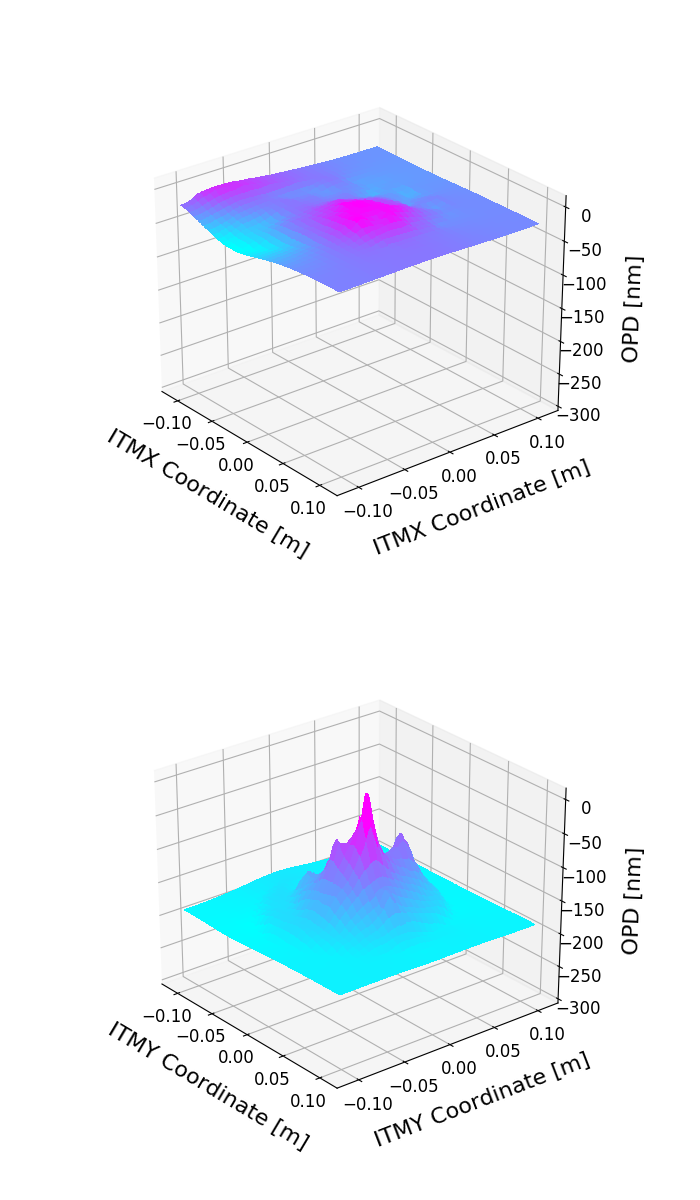
\includegraphics[width=0.4\textheight]{../Figures/1231726400_3d_500dur_30W_ITM.png}\quad
	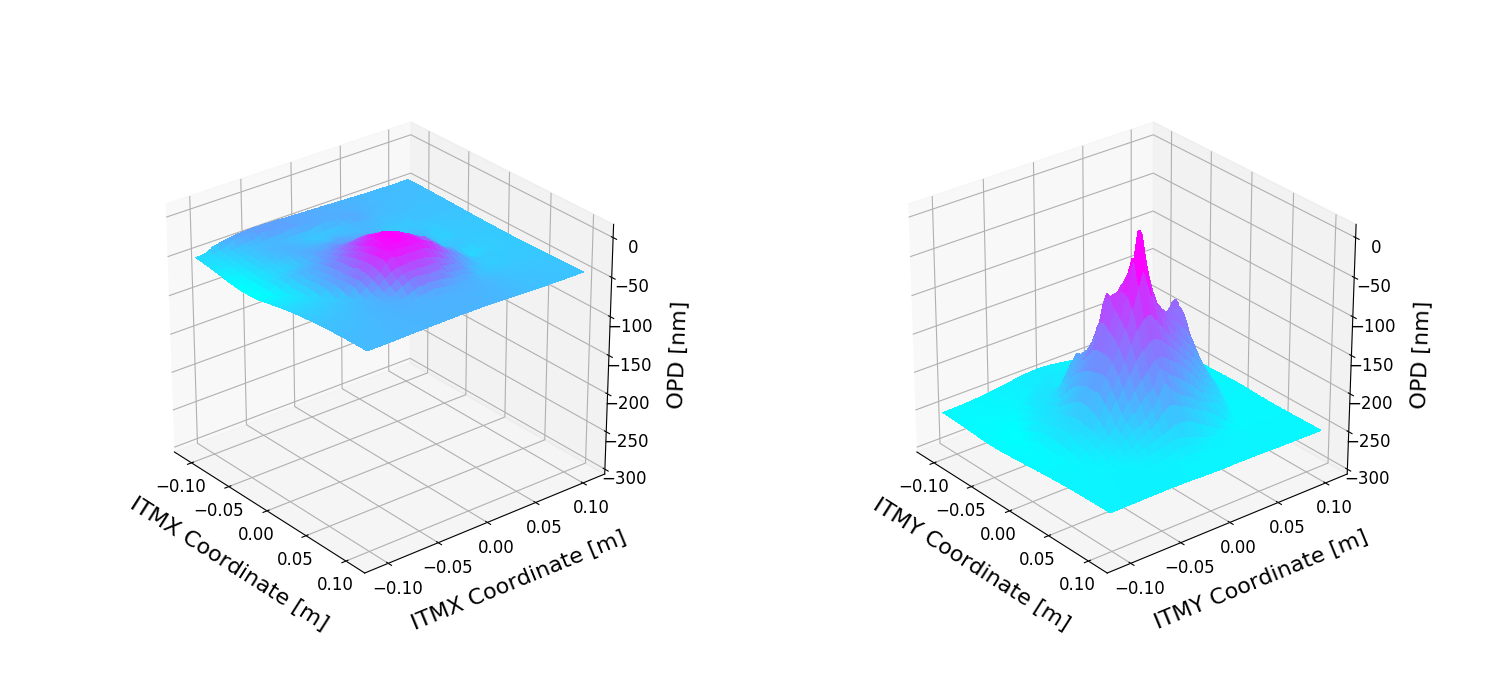
\includegraphics[width=0.4\textheight]{../Figures/1231726400_3d_1000dur_30W_ITM.png}\quad
	\caption[Comparing 3-D plots of the optical path distortion for ITMX and ITMY test masses after powering up the interferometer.]  
	{\textbf{Comparing 3-D plots of the optical path distortion for ITMX and ITMY test masses after powering up the interferometer.}
		The horizontal axes represent the test mass coordinates as seen on the Hartmann sensors and the vertical axis is the optical path distortion in units of nanometers. The color map is scaled for each plot and is meant to show particularly hot areas and roughly compare the high frequency spatial distribution of point absorbers. Plots in the left column (ITMX) have smooth spatial features that stem from uniform absorption and the effects are not prominent till after approximately 500 seconds.  In contrast, plots in the right column (ITMY) have very sharp spatial features which already rise above the floor at 200 seconds into powering up.  Comparing the overall surface deformation on the same scale, the difference between ITMX and ITMY is striking and it is clear how an interferometer with point absorbers on the surface will struggle to increase powers above 200 kW within the arm cavities.
	}
	\label{fig:3d_HWS_plot}
\end{figure}

\begin{figure}[ht]
	\centering
	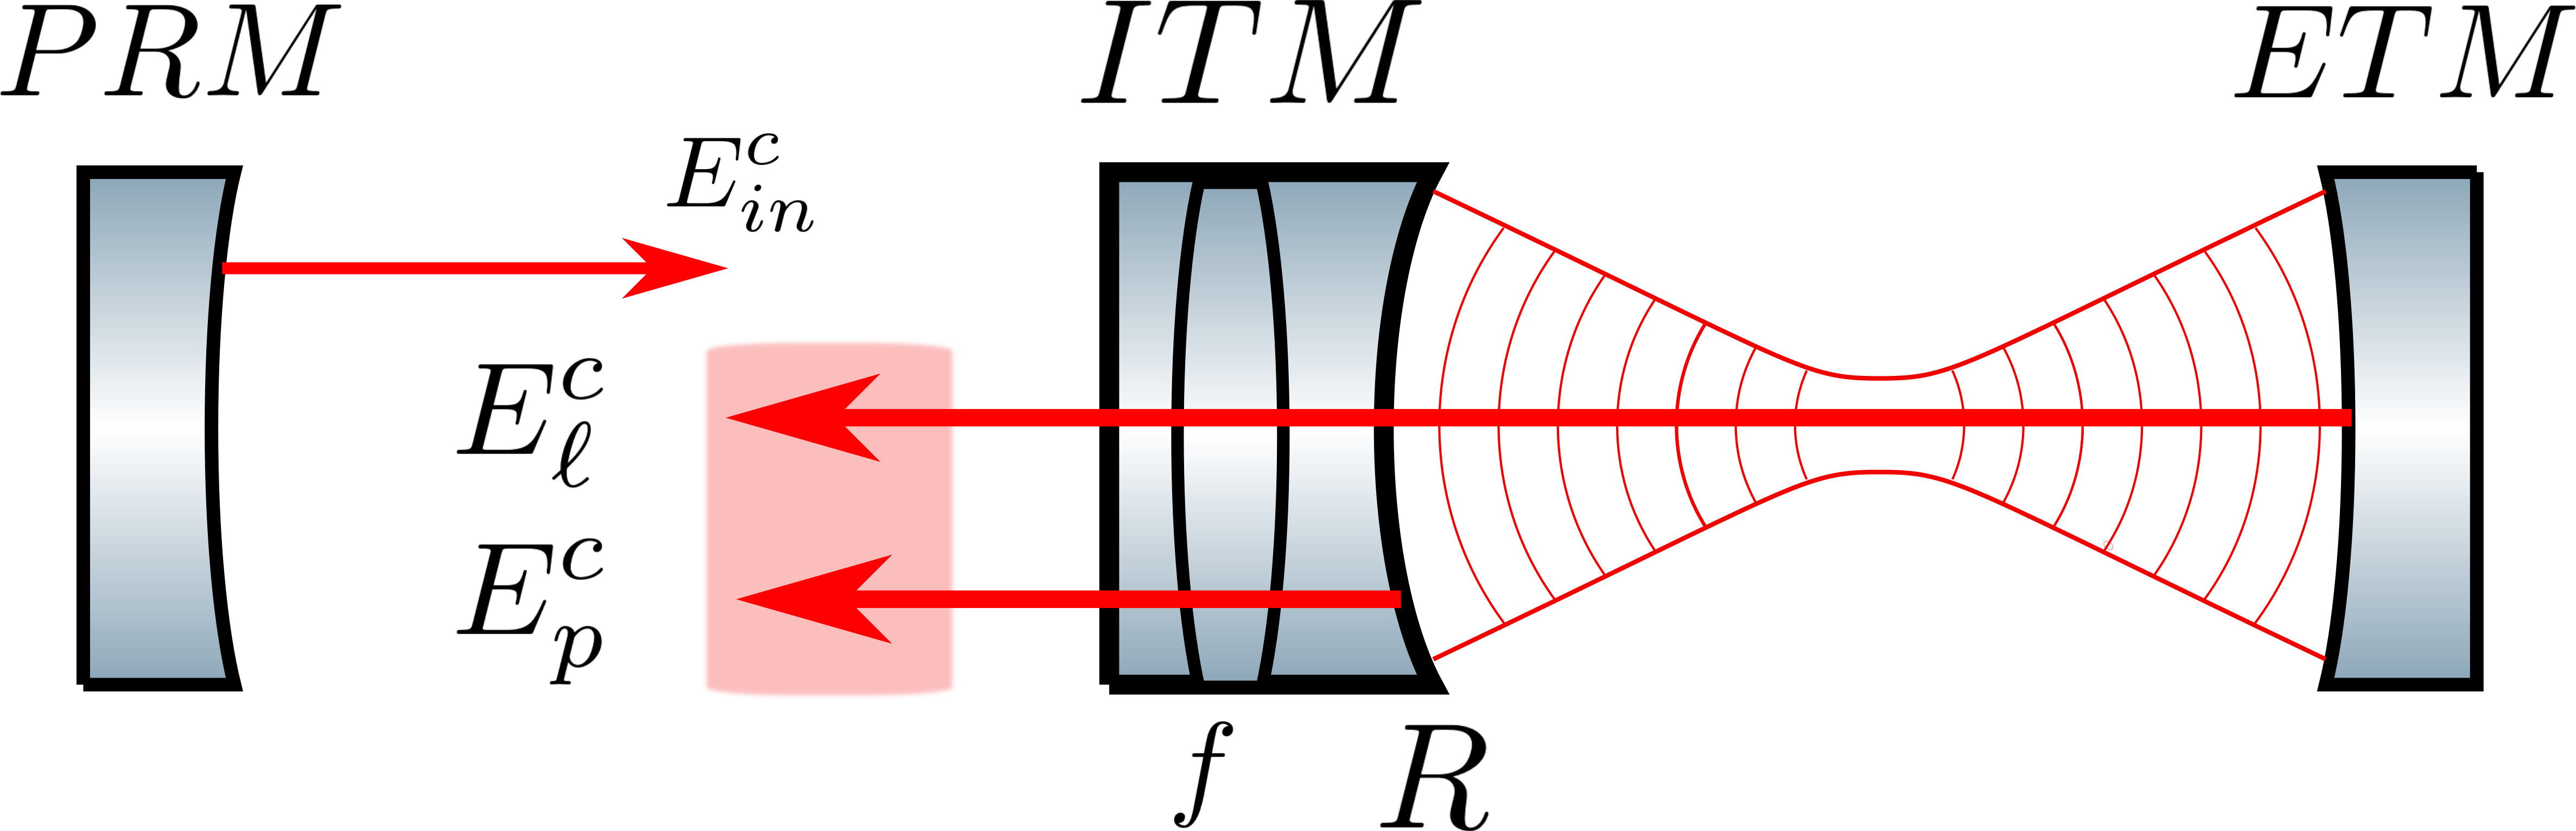
\includegraphics[width=.7 \textwidth]{../Figures/ThermalLensFP.png}
	\caption[A simplified model for the effect of a substrate thermal lens on the carrier field.]  
	{\textbf{A simplified model for the effect of a substrate thermal lens on the carrier field.} An input beam, $E_{\text{in}}^{c}$, from the power recycling mirror (PRM) will have a radius of curvature that mode matches to the input test mass (ITM).  The promptly reflected beam, $E_{p}^{c}$, is denoted by equation \ref{eq:promptE} and the leakage beam, $E_{\ell}^{c}$, is expressed by equation \ref{eq:leakE} where the sum of them would make the total reflected beam.  The leakage field will have the same shape as the ITM radius of curvature $R$ when exiting the arm and see the thermal lensing $f$. The promptly reflected field will also see the lens $f$ twice but when combined with the leakage beam, the \textit{total} reflected field is not affected by the thermal lens.}
	\label{fig:ThermalLensFP}
\end{figure}

\begin{figure}[ht]
	\centering
	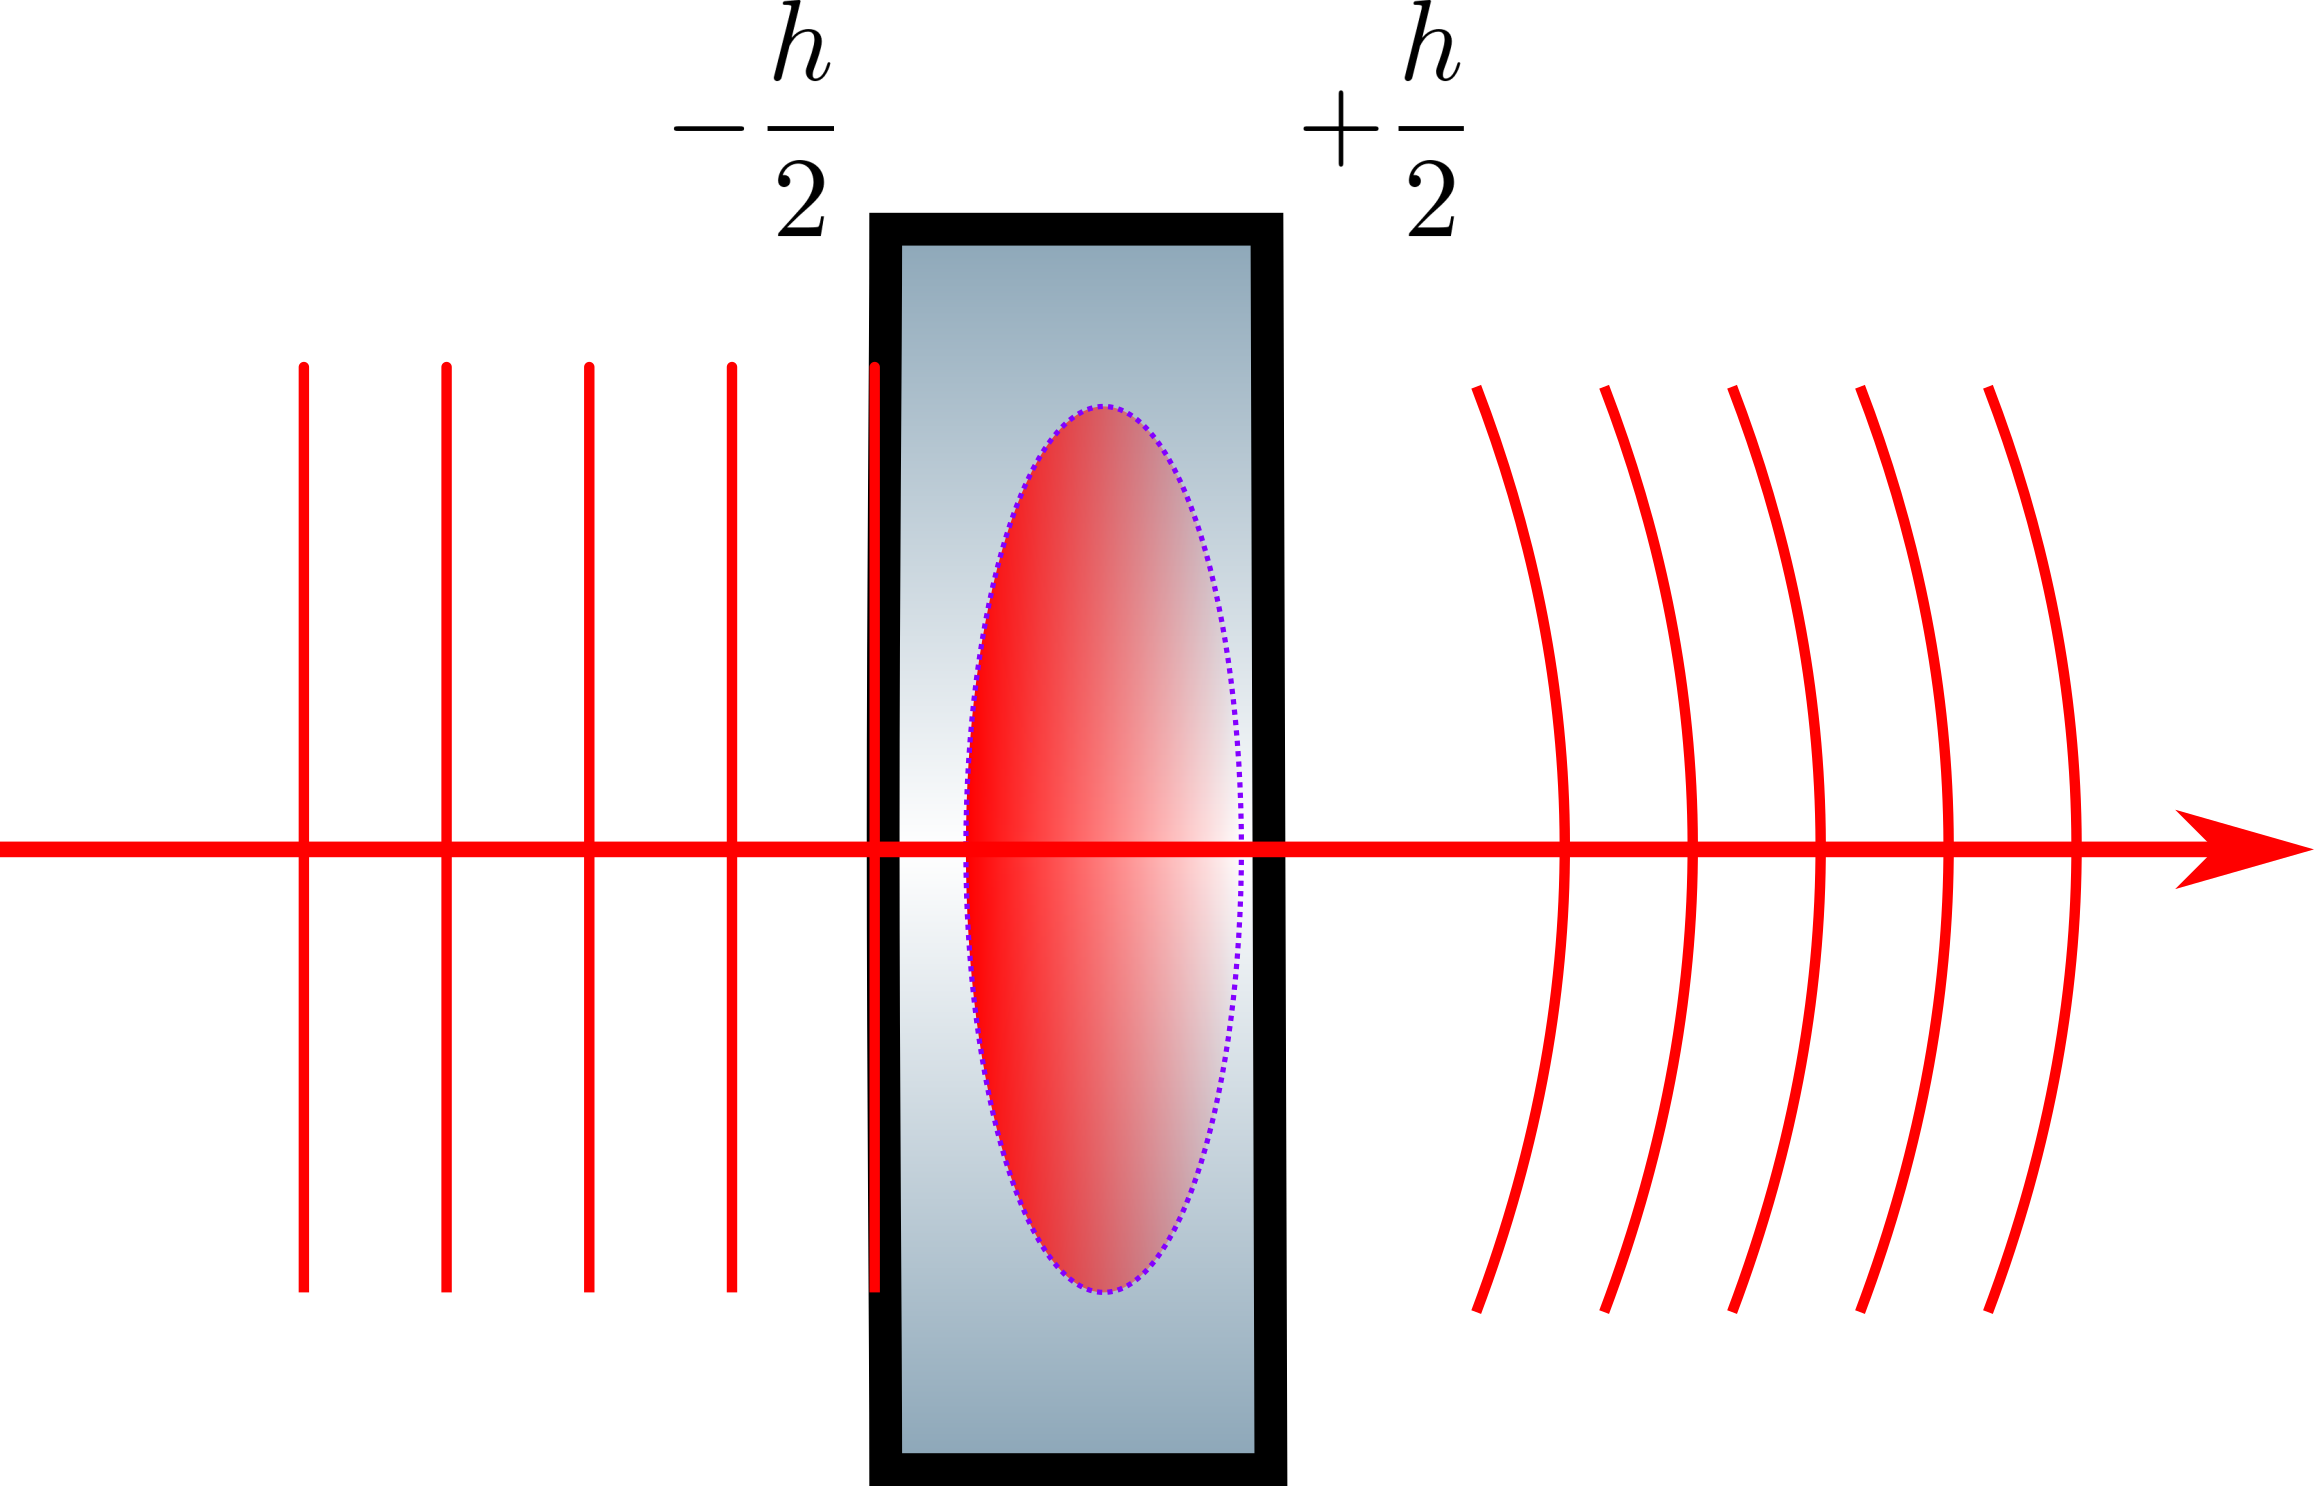
\includegraphics[width=.4 \textwidth]{../Figures/ThermalLensWF.png}
	\caption[A plane wave passing through a lens with a temperature gradient.]  
	{\textbf{A plane wave passing through a lens with a temperature gradient.} The index of refraction, $n$, depends on the material and temperature field, when a plane wave moves through such a lens, then a phase lag or lead occurs in the wavefront. Since $\frac{\text{d}n}{\text{d}T}$ is negative, the thermal distortion will resemble a diverging lens.}
	\label{fig:ThermalLensWF}
\end{figure}

\begin{figure}[ht]
	\centering
	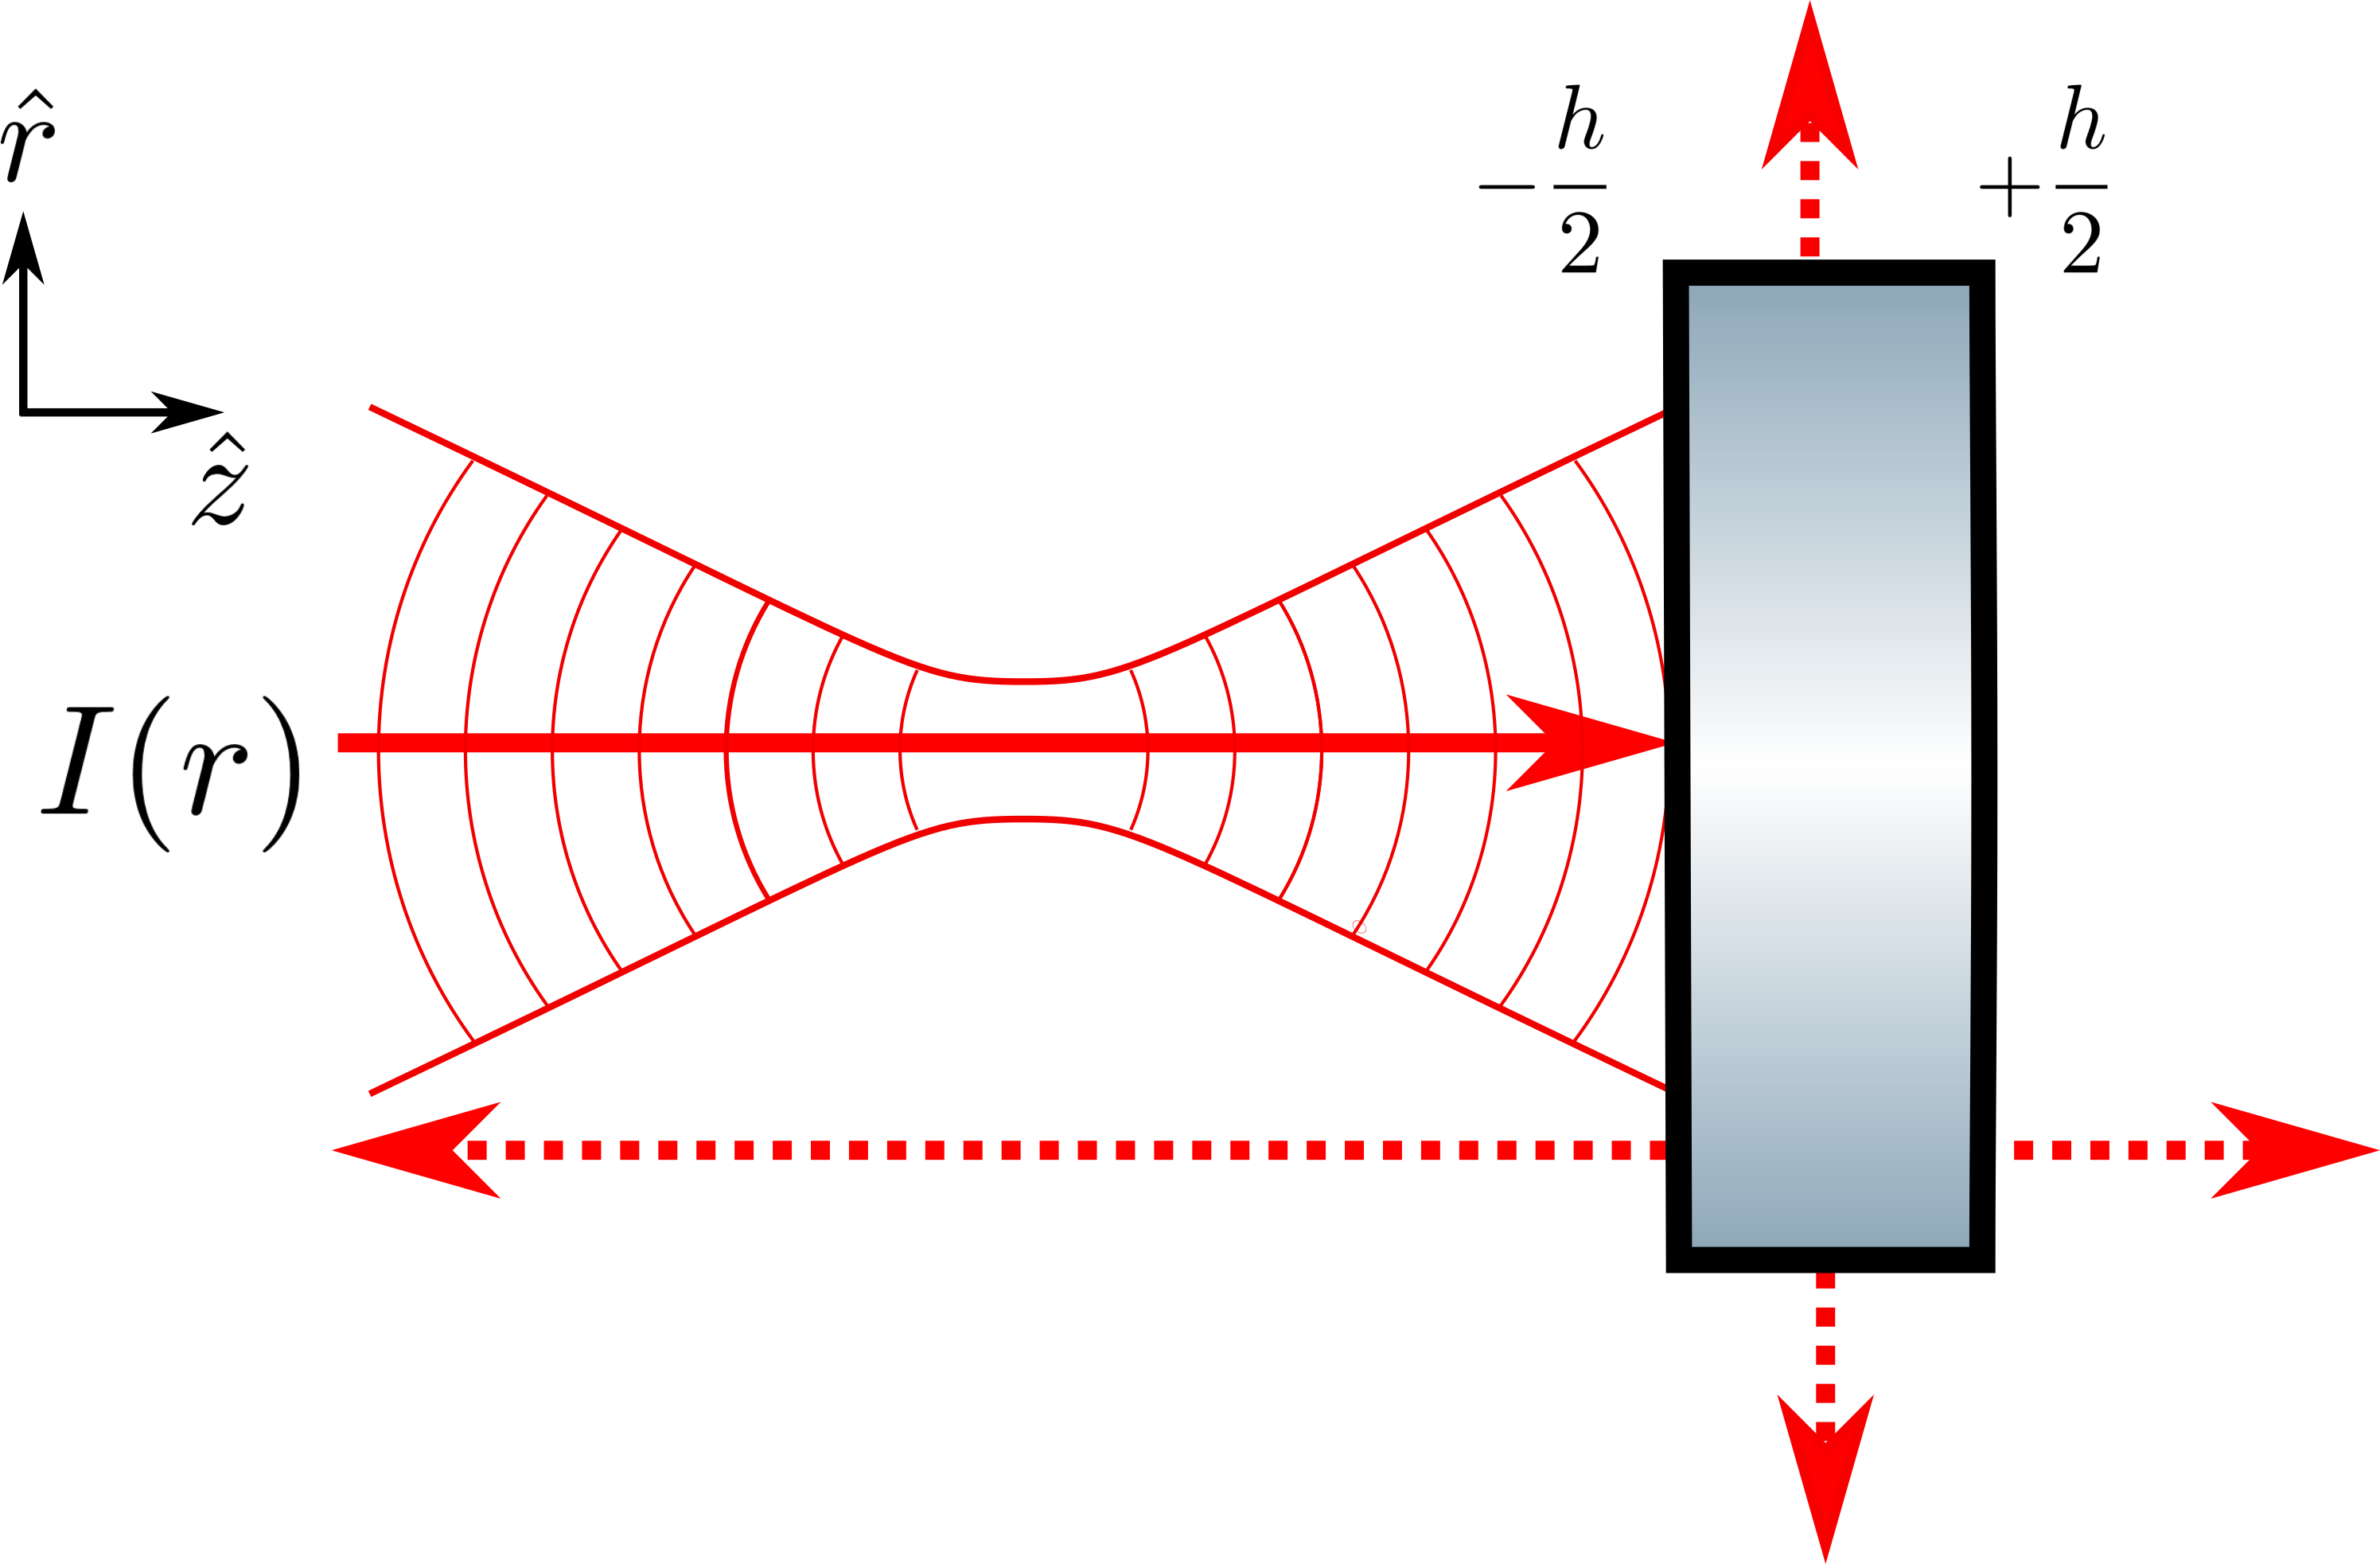
\includegraphics[width=.6 \textwidth]{../Figures/ThermalLensFlux.png}
	\caption[A conceptual model of flux balance for a cylindrical object.]  
	{\textbf{A conceptual model of flux balance for a cylindrical object.} The red dotted lines represent the radiative fluxes escaping the optic while a Gaussian beam with intensity profile $I(r)$ is pumping energy in as denoted by the red solid line.}
	\label{fig:ThermalLensFlux}
\end{figure}


\begin{figure}[ht]
	\centering
	\begin{subfigure}[a]{0.7\textwidth}
		\centering
		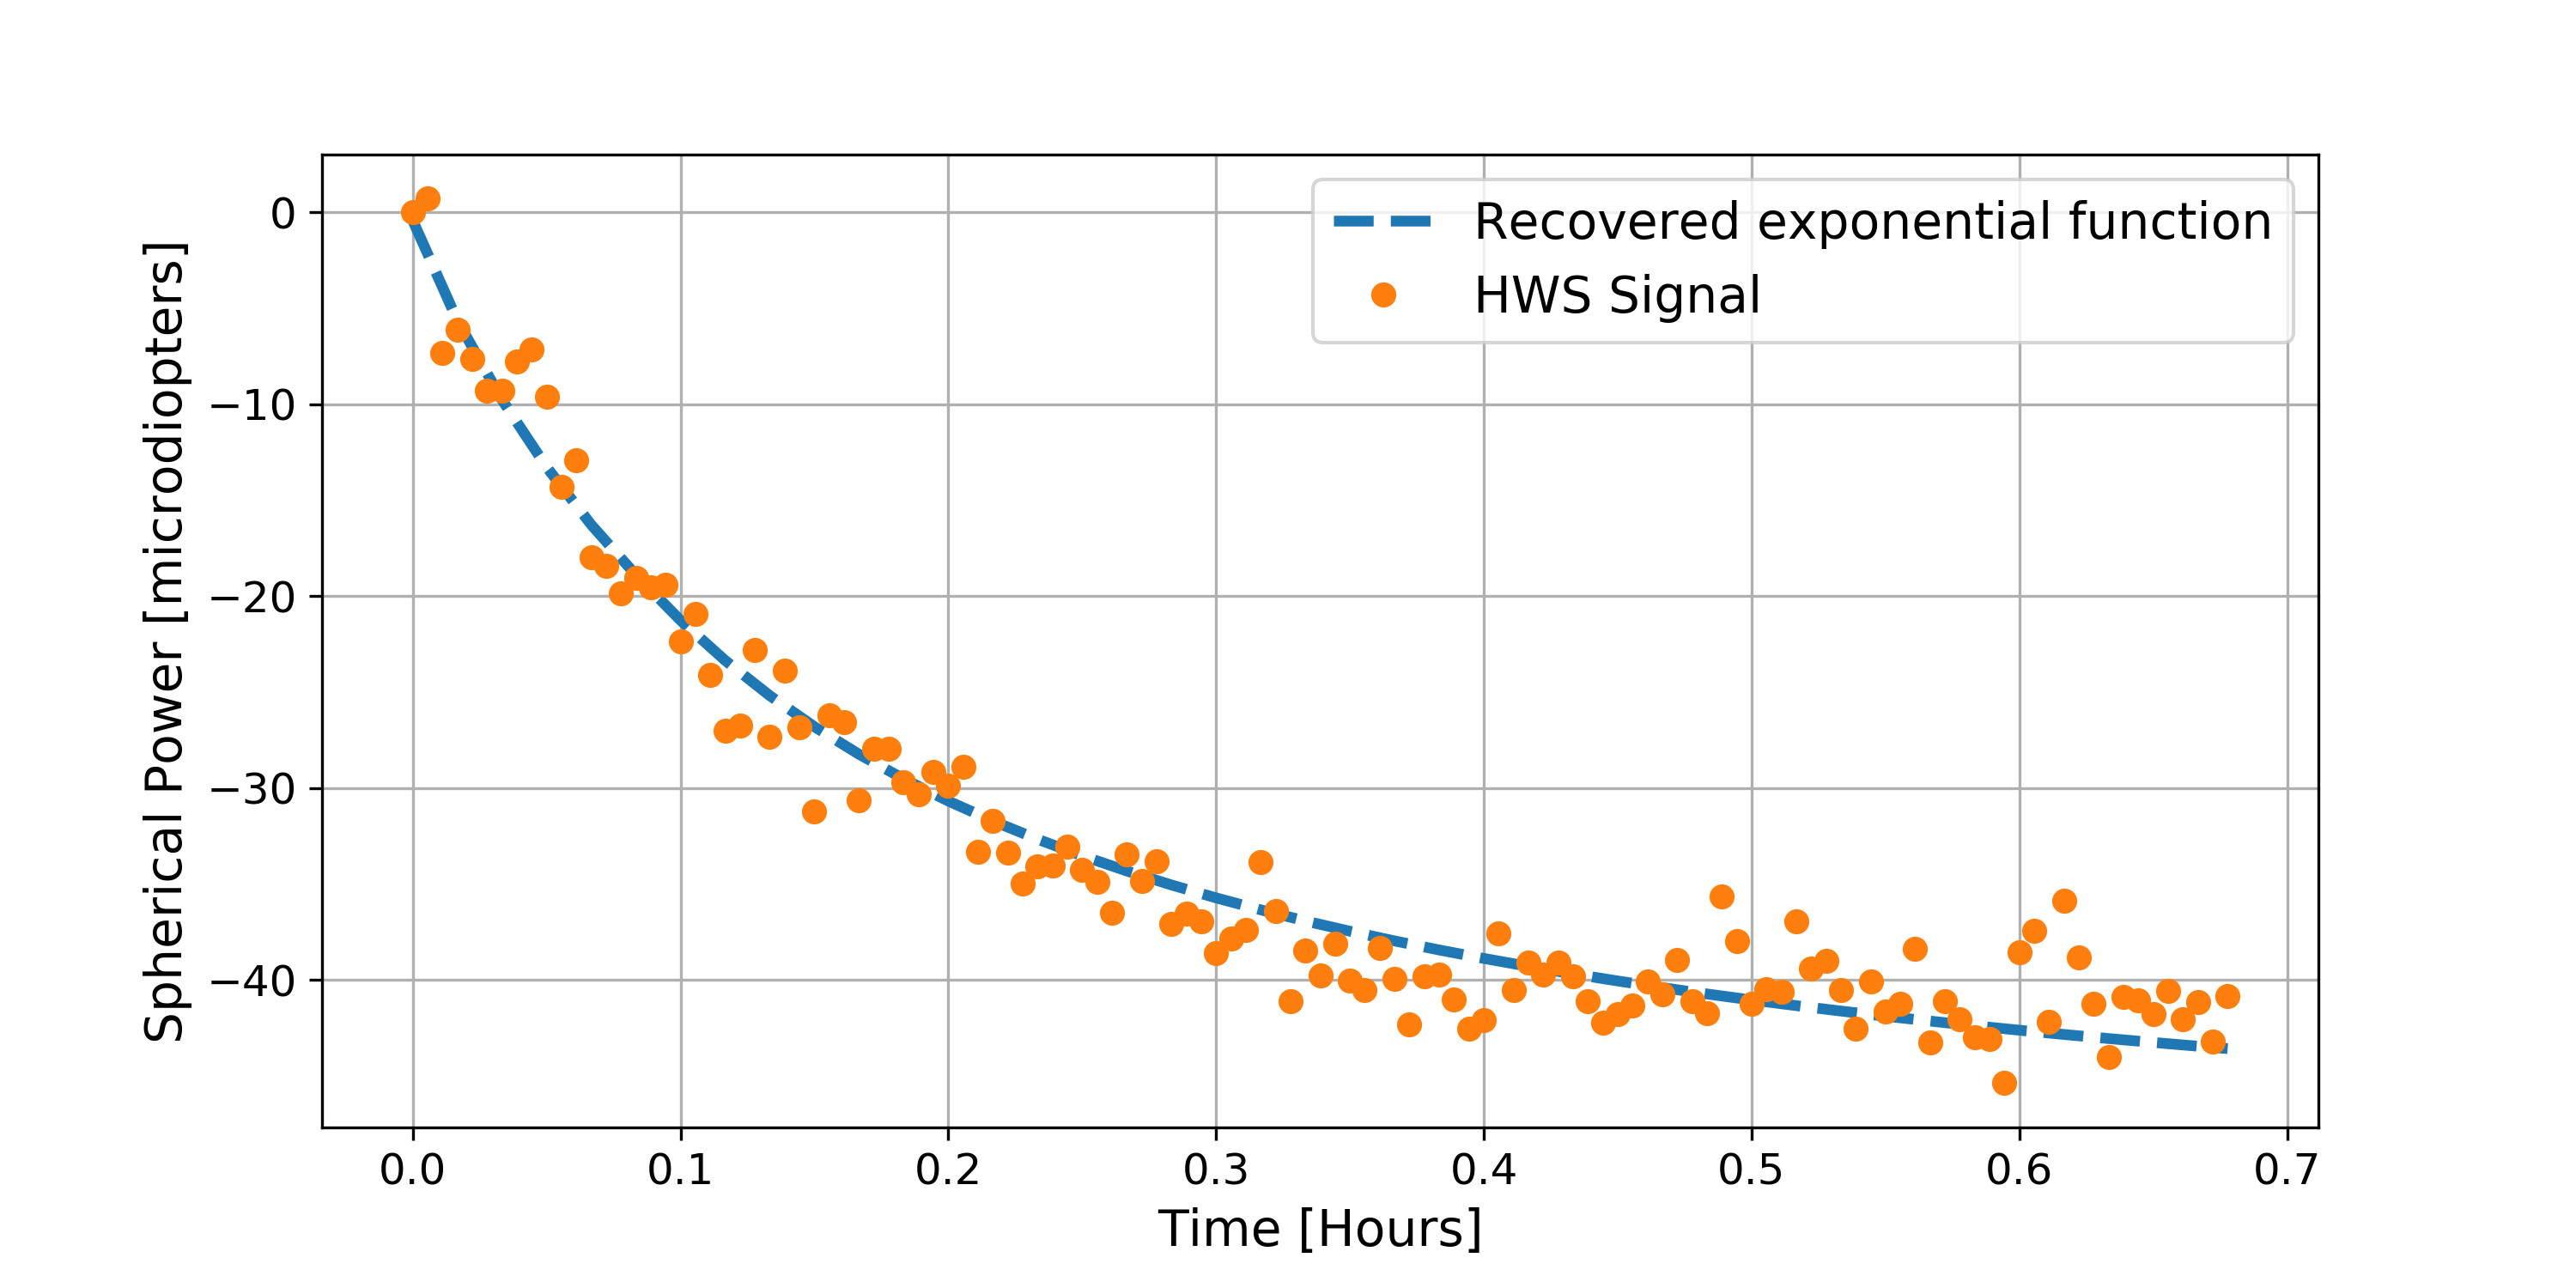
\includegraphics[width=\textwidth]{../Figures/MCMC_ITMX_ABS_FIT.png}
		\caption{ITMX absorption}
		\label{fig:itmx_abs}
	\end{subfigure}
	\hfill
	\begin{subfigure}[b]{0.7\textwidth}
		\centering
		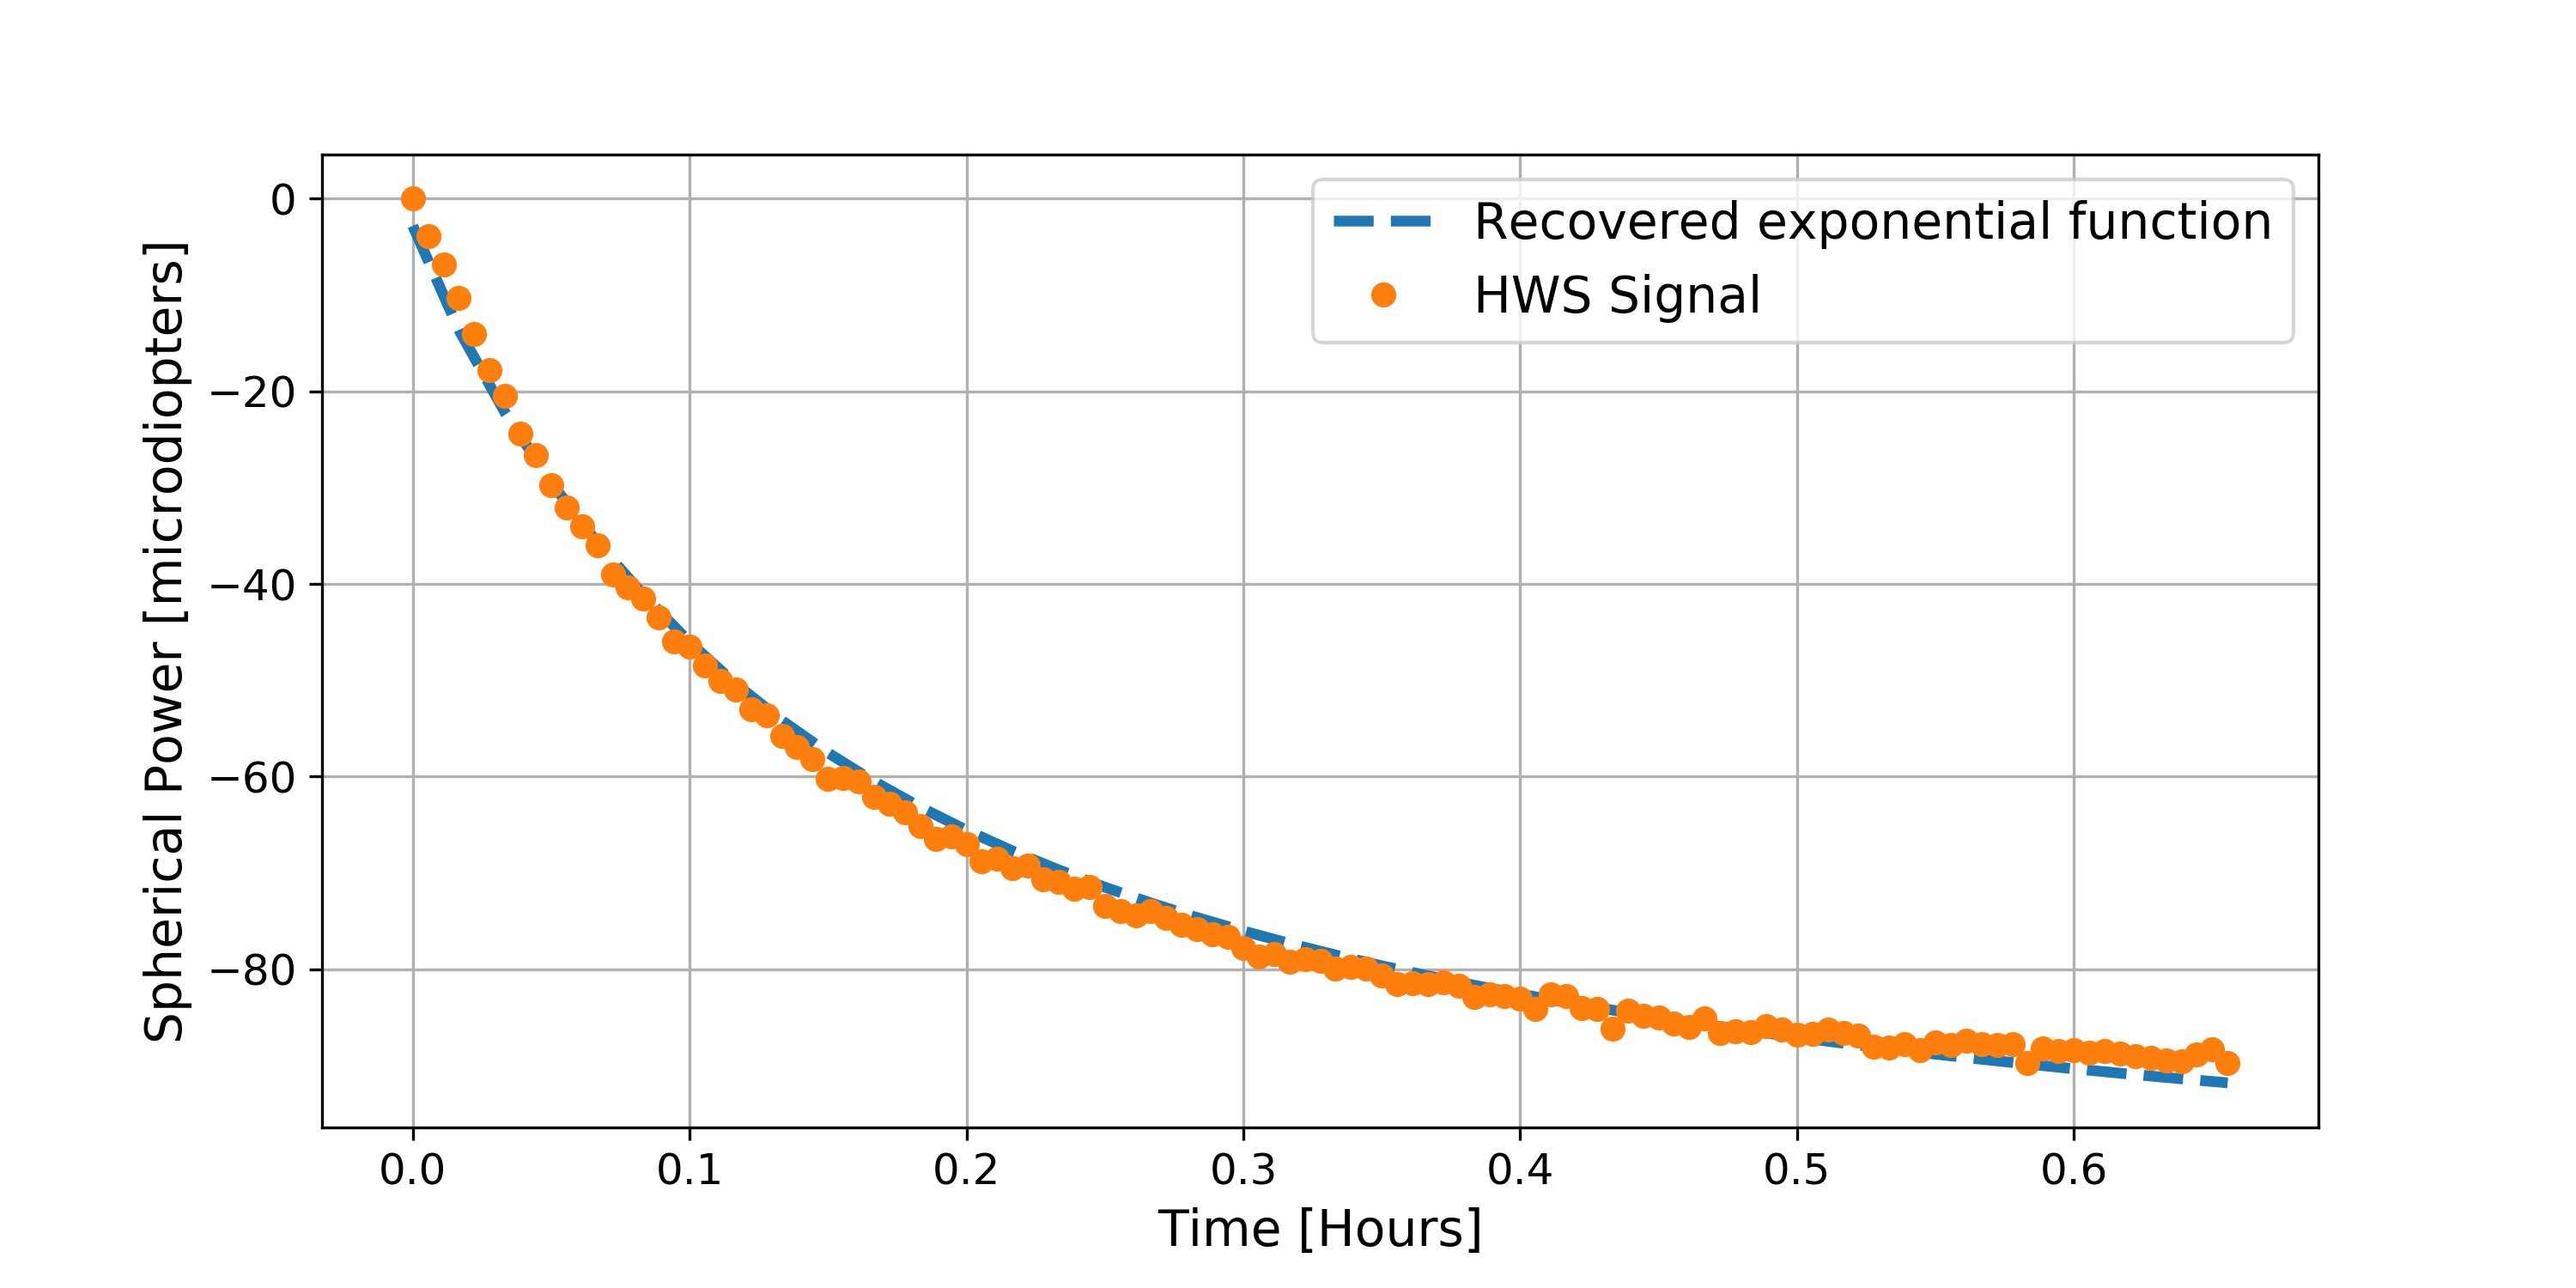
\includegraphics[width=\textwidth]{../Figures/MCMC_ITMY_ABS_FIT.png}
		\caption{ITMY absorption}
		\label{fig:itmy_abs}
	\end{subfigure}
	\caption[Thermal lensing as seen by the ITM Hartmann Sensors after a lock loss.]  
	{\textbf{Thermal lensing as seen by the ITM Hartmann Sensors after a lock loss.} A finite element model from COMSOL shows an exponential decay which can be linearized and fitted to the spherical power. Comparing ITMX and ITMY at Hanford shows a huge overall difference between the two optics, mostly due to the fact that ITMY has multiple point absorbers adding to the absorption estimate.}
	\label{fig:hws_abs}
\end{figure}

\begin{figure}[ht]
	\centering
	\begin{subfigure}[b]{0.5\textwidth}
		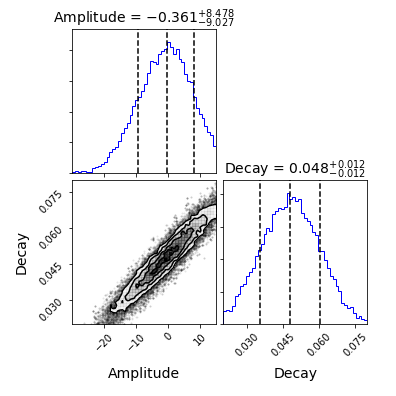
\includegraphics[width=\linewidth]{../Figures/MCMC_ITMX_abs.png}
		\caption{ITMX}
		\label{fig:mcmc_itmx_abs}
	\end{subfigure}%
	\begin{subfigure}[b]{0.5\textwidth}
		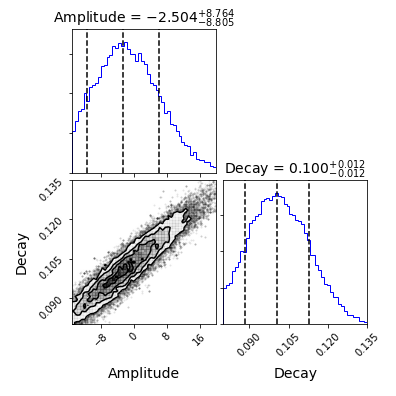
\includegraphics[width=\linewidth]{../Figures/MCMC_ITMY_abs.png}
		\caption{ITMY}
		\label{fig:mcmc_itmy_abs}
	\end{subfigure}
	\caption[Posterior distributions from fitting the Hartmann sensor spherical power.]  
	{\textbf{Posterior distributions from fitting the Hartmann sensor spherical power.}  
	Using the MCMC Hammer \cite{MCMC_Hammer}}
	\label{fig:mcmc_hws_abs}
\end{figure}

\begin{figure}[ht]
	\centering
	\begin{subfigure}[b]{1.0\textwidth}
		\centering
		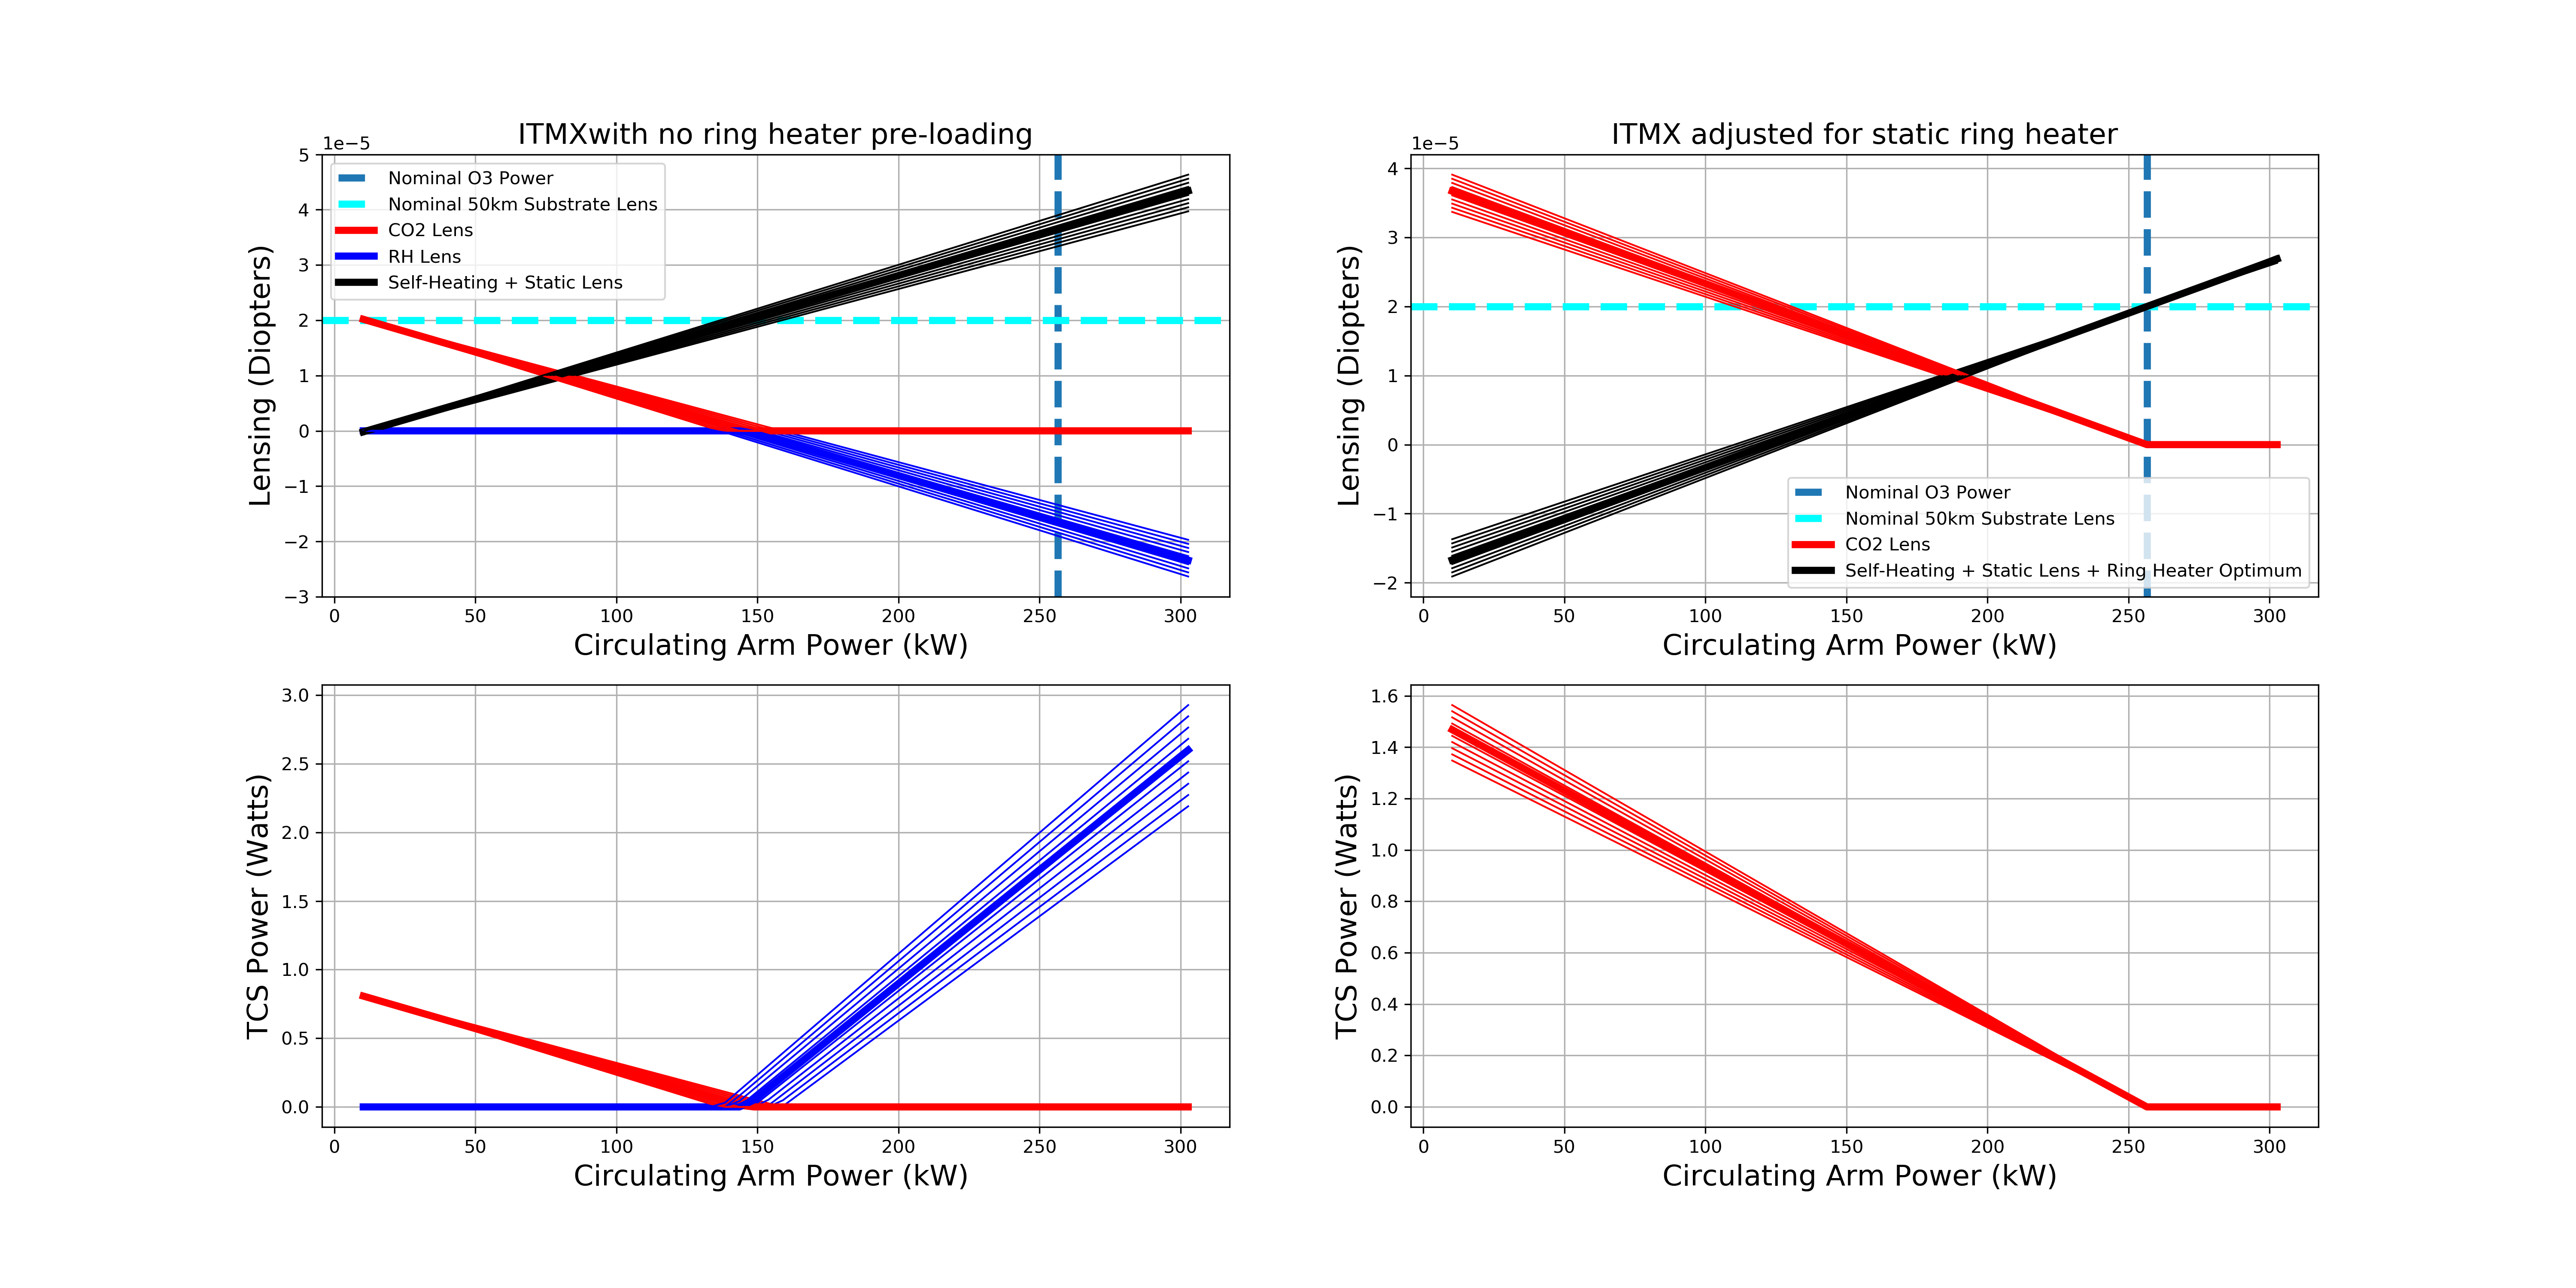
\includegraphics[width=\textwidth]{../Figures/ITMX_TCS_Settings.png}
		\label{fig:TCS_ITMX}
	\end{subfigure}
	\hfill
	\begin{subfigure}[b]{1.0\textwidth}
		\centering
		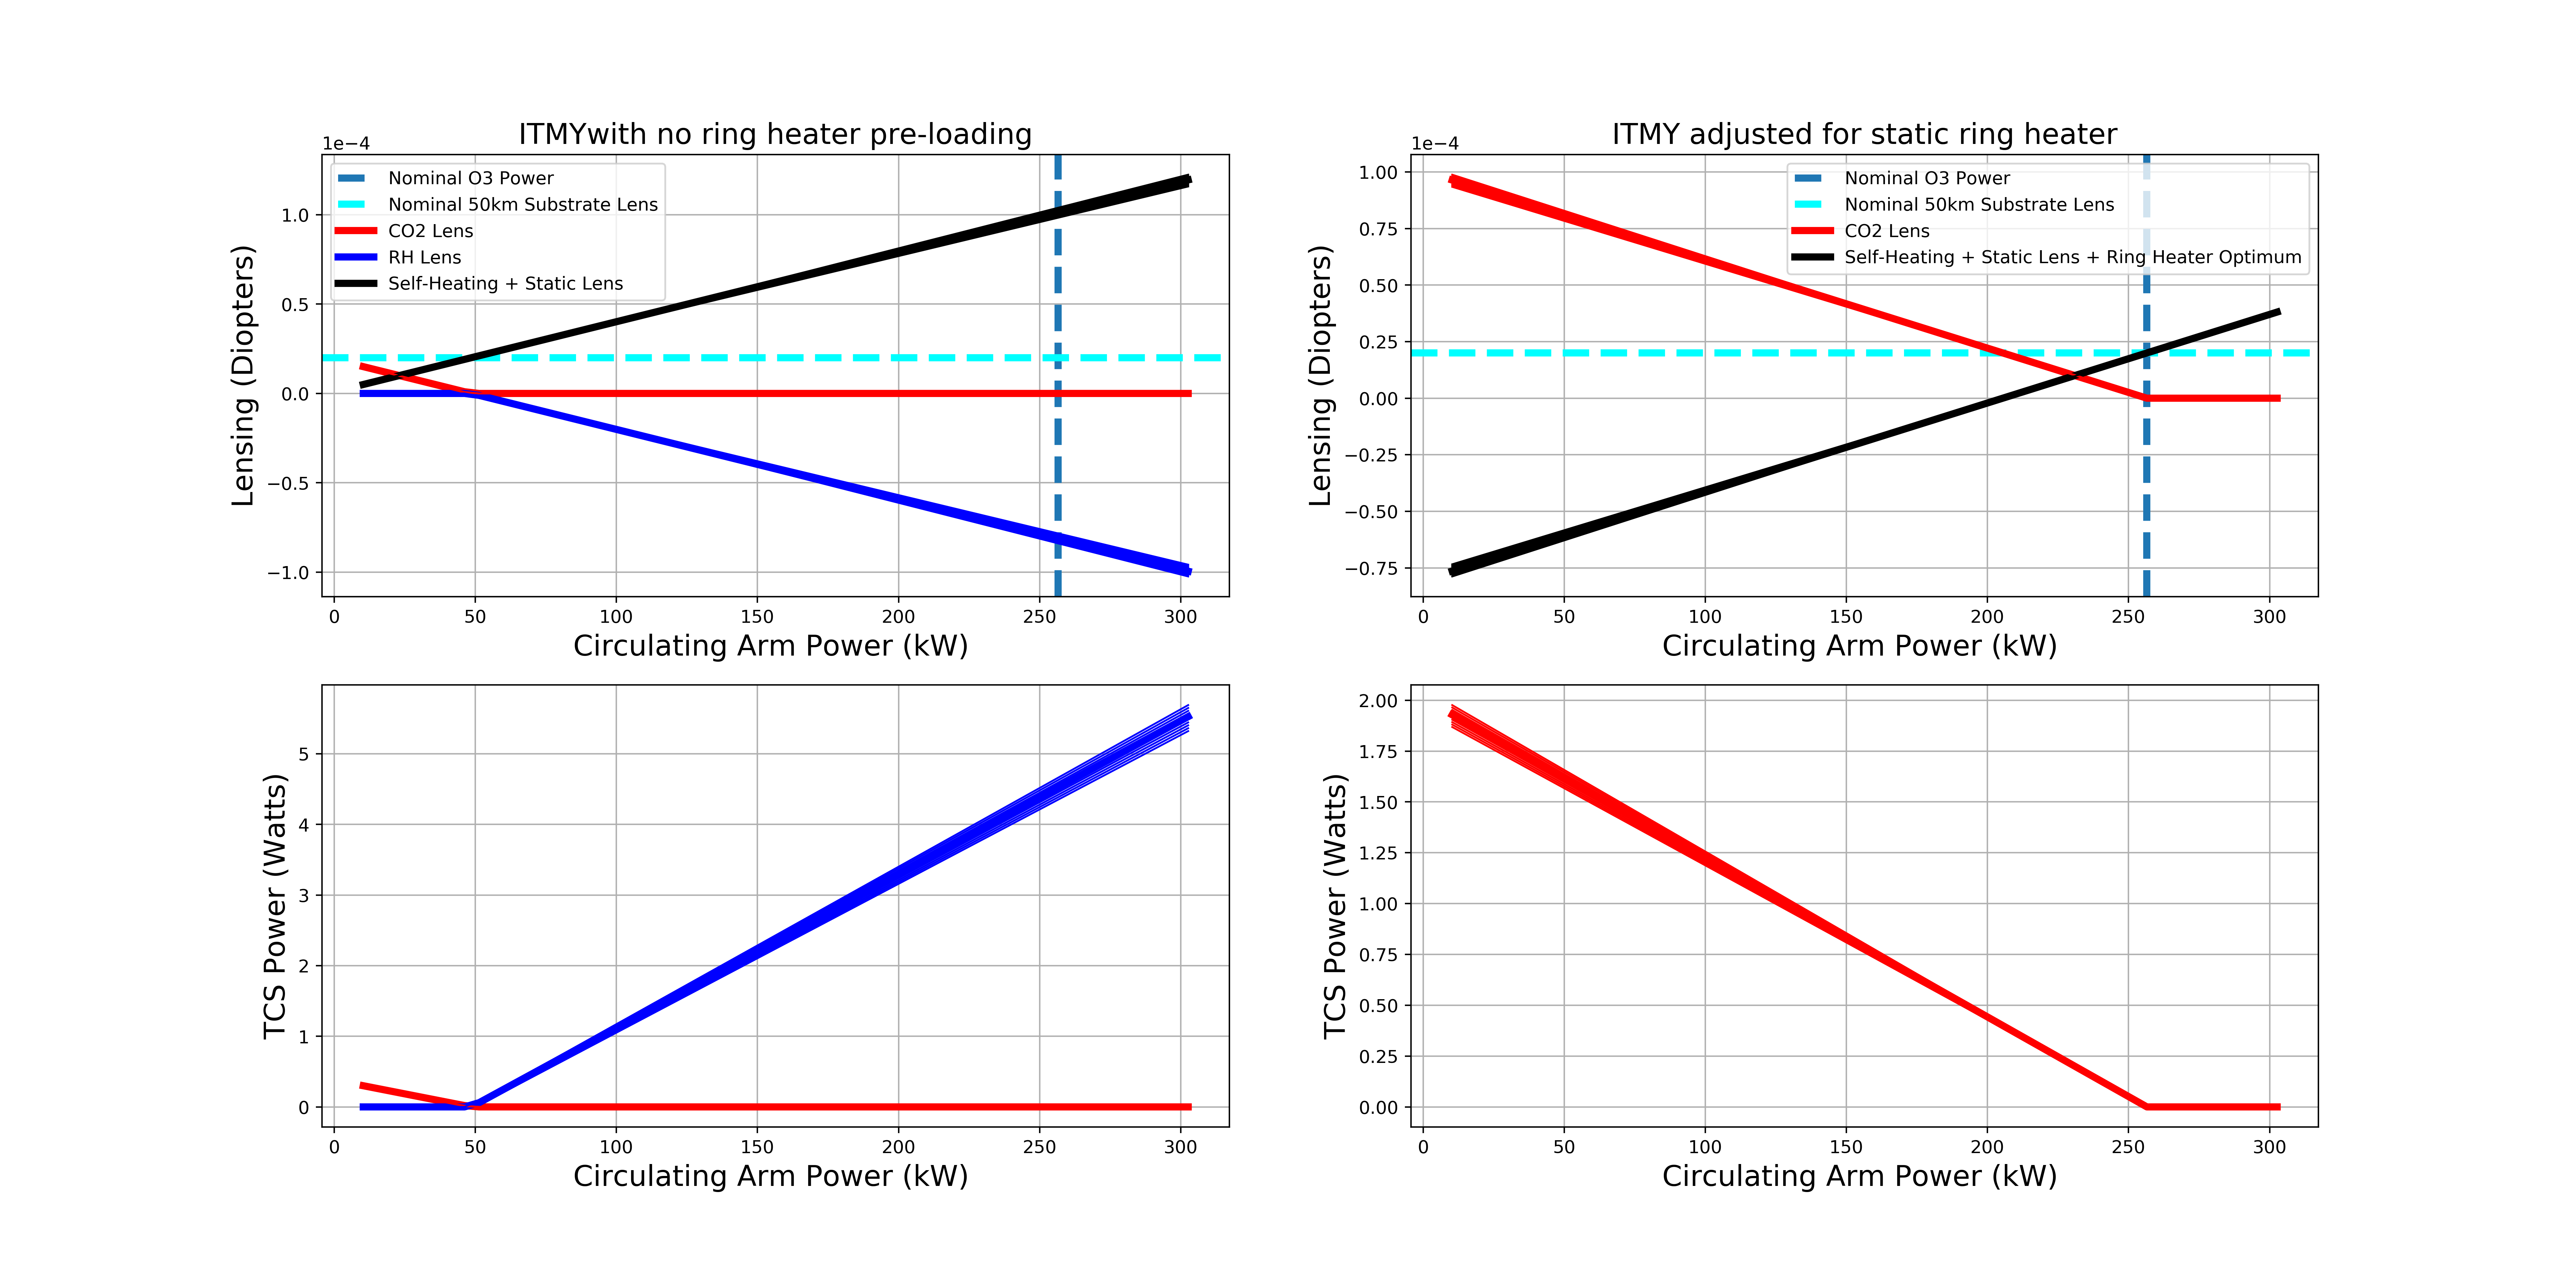
\includegraphics[width=\textwidth]{../Figures/ITMY_TCS_Settings.png}
		\label{fig:TCS_ITMY}
	\end{subfigure}
	\caption[Calculated TCS settings to balance the substrate lens.]{
		\textbf{Calculated TCS settings to balance the substrate lens.}  The nominal circulating power denoted by the vertical blue line is a function of the input power, the recycling gain, and the arm cavity gain.  The nominal input power for O3 will be 50 Watts and the power recycling gain is around 45.  The arm cavity gain can be estimated by calibrating the transmitted power from each of the arms and is approximately 228.  The horizontal, dashed turquoise line represents the nominal substrate lens with a focal length of 50 km.  This value is what the power recyling cavity expects to properly mode match to the arms. 
	}
	\label{fig:TCS_ITMs}
\end{figure}

\begin{figure}[ht]
\centering
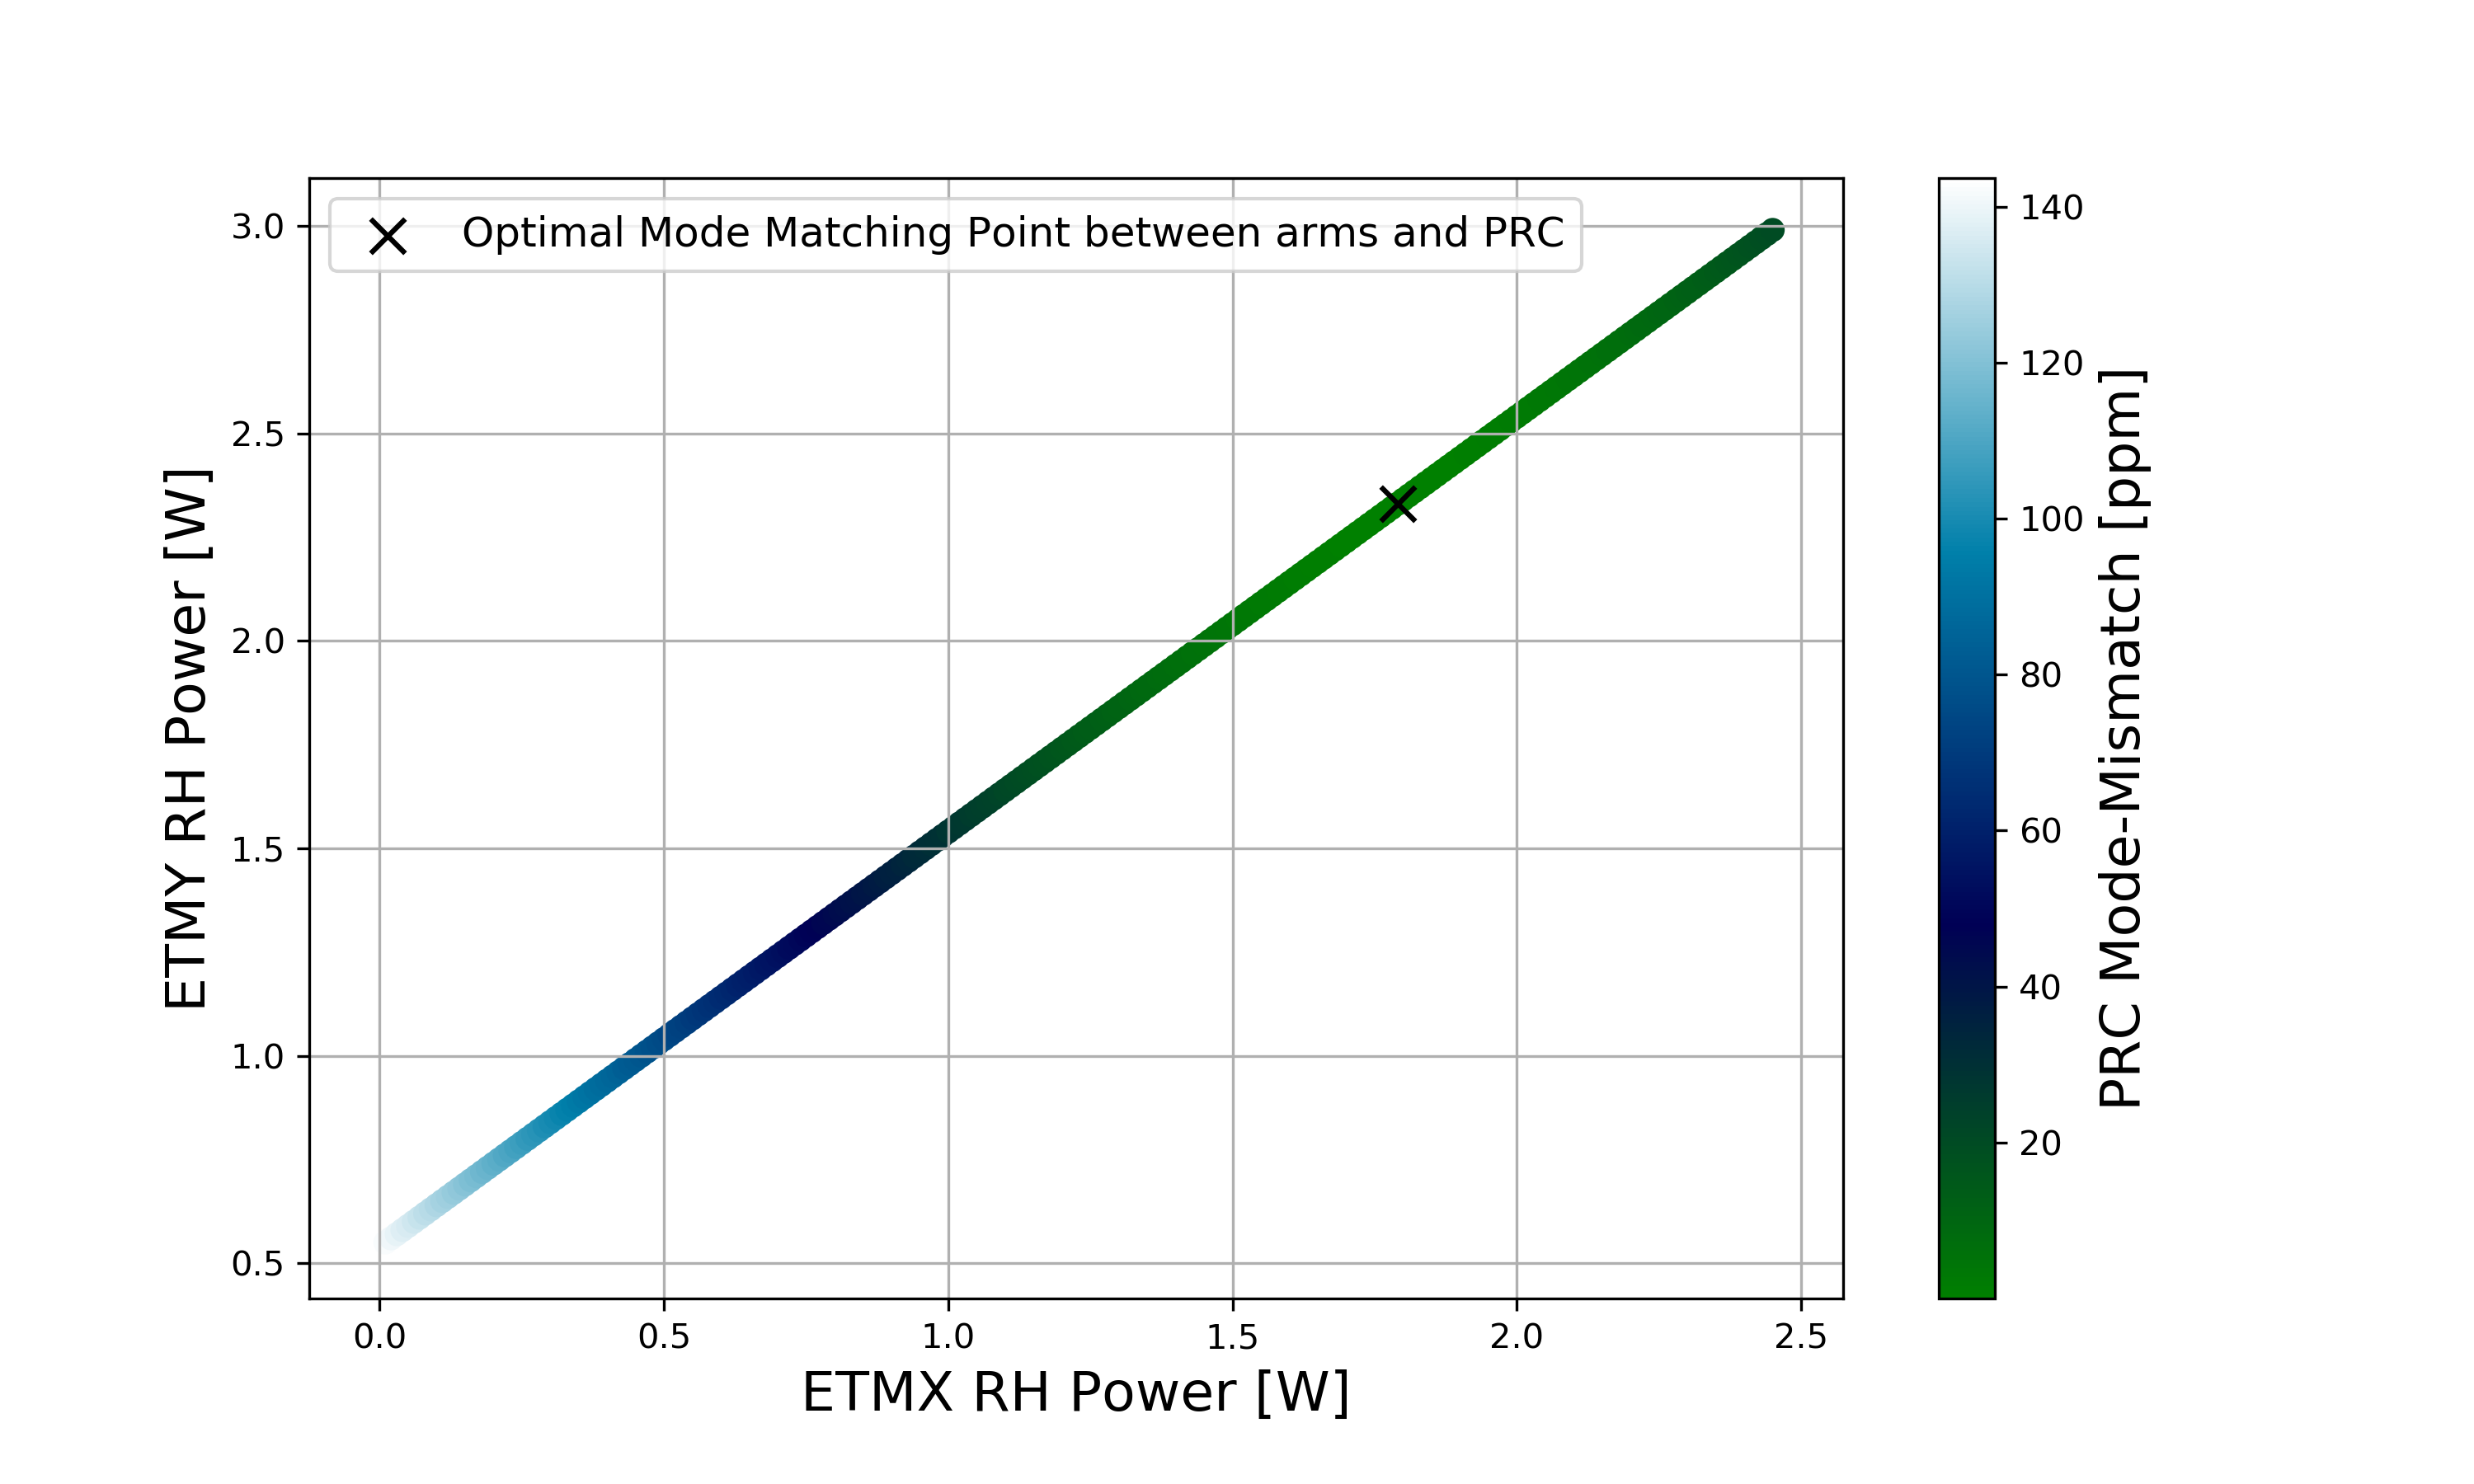
\includegraphics[width=1.0 \textwidth]{../Figures/ETM_TCS_Settings.png}
\caption[Mode matching the arm cavities to the power recycling cavity.]{
	\textbf{Mode matching the arm cavities to the power recycling cavity.}  Determining the ITM ring heaters and CO2 power levels still leaves the end test mass ring heaters to be set.  The goal is to maintain the mode matching between the arms while simultaneously searching for the optimal overlap with the power recycling cavity.  This is done by determining the spatial mode overlap between all three cavities (2 ARMS) The linear portion of the graph shows a combination of common and differential adjustment of each ring heater that keeps the mode matching between the arms at less than 1 PPM 
	}
\label{fig:TCS_ETM}
\end{figure}